The aim of this project was to obtain an x-ray image of a 3D printed sample and compare it with a simulation of that scan using software called \texttt{aRTist} \citep{bellon2007artist, jaenisch2008artist, bellon2012radiographic}. \texttt{aRTist} can simulate x-ray scans of the 3D printed sample given the specifications of the scan, such as the x-ray source, the x-ray detector and the blueprint of the 3D printed sample \citep{bellon2011simulation, deresch2012simulating}. Users of \texttt{aRTist} can align the simulated x-ray image to the real x-ray image using numerical methods, however this is outside the scope of this thesis.

Disagreement between the scan and \texttt{aRTist} can be found by simply subtracting one image from the other, any values too big in magnitude can be considered as a defect. However in the previous chapters, it was found that x-ray photons behave randomly and differences in the comparison can be due to chance. Thus the comparisons should be done under the face of uncertainty.

A pixel by pixel inference was proposed to do defect detection. A statistic $z_{x,y}$ for the $(x,y)$ positioned pixel was calculated for all pixels. This statistic is
\begin{equation}
    Z_{x,y} = 
    \dfrac{
        \text{scan}_{x,y} - \text{aRTist}_{x,y}
    }
    {
        \sqrt{\widehat{\variance}\left[\text{scan}_{x,y}\right]}
    }
\end{equation}
where $\widehat{\variance}\left[\text{scan}_{x,y}\right]$ is the estimated grey value variance of pixel $(x,y)$ in the scan. Under mild assumptions, it was shown in the previous chapters that the grey values in the scan were Normal. Thus by treating the simulated image from \texttt{aRTist} as known and the ground truth, then the randomness of the $z_{i,j}$ statistics can be quantified
\begin{equation}
Z_{i,j}\sim \normal(0,1) \ .
\end{equation}
As with usual statistical convention, upper case $Z$ denote a random variable. Whereas lower case $z$ denote a realisation or an observation of that random variable.

The estimation of the grey value variance, that is $\widehat{\variance}\left[\text{scan}_{i,j}\right]$ is be explained here. The variance model can be calibrated, or trained, by holding out a number replicated x-ray scans of a 3D printed sample. These replicated x-ray scans provide variance-mean data which was used to train the variance model, such as a Gamma distributed GLM. The method on doing so was described in the previous chapter and it was found a linear relationship between the variance and the mean was a good model. The variance was then predicted using the grey value in the \texttt{aRTist} simulation.

This method for inference was applied to the dataset \texttt{Sep16 120deg}. Here a cuboid with voids were purposefully manufactured to see if they can be detected. The 20 x-ray images were spilt into 2. 19 images were used to train the variance-mean model. One image, called the test image, was used to compare with \texttt{aRTist}, as shown in Figure \ref{fig:inference_initial_artist_scan_aRTist}. In the \texttt{aRTist} simulation, the software did a simulation as if the voids were not there. 

\begin{figure}
	\centering
    \centerline{
    \begin{subfigure}[b]{0.49\textwidth}
        \includegraphics[width=\textwidth]{../figures/inference/initial_artist_scan.eps}
        \caption{X-ray image}
    \end{subfigure}
    \begin{subfigure}[b]{0.49\textwidth}
        \includegraphics[width=\textwidth]{../figures/inference/initial_artist_aRTist.eps}
        \caption{\texttt{aRTist} simulation}
    \end{subfigure}
    }
    \caption{An x-ray scan of a 3D printed cuboid, from the \texttt{Sep16 120deg} dataset. This can be compared directly to the \texttt{aRTist} simulation for defects.}
    \label{fig:inference_initial_artist_scan_aRTist}
\end{figure}

For each pixel, a $z$ statistic was calculated. A $z$ statistic too large in magnitude can be considered to be evidence of a positive result. Another way to represent the $z$ statistic is the $p$-value which is given as
\begin{equation}
    p_{x,y} = 2(1-\Phi(\|z_{x,y}\|))
\end{equation}
which can takes values $0\leqslant p_{i,j} \leqslant 1$. A $p$-value too small is considered to be evidence of a defect. The resulting $z$ statistics and $p$-values are shown in Figure \ref{fig:inference_initial_artist_logp_z}.

\begin{figure}
	\centering
    \centerline{
    \begin{subfigure}[b]{0.49\textwidth}
        \includegraphics[width=\textwidth]{../figures/inference/initial_artist_logp.eps}
        \caption{$-\log p\text{-values}$}
    \end{subfigure}
    \begin{subfigure}[b]{0.49\textwidth}
        \includegraphics[width=\textwidth]{../figures/inference/initial_artist_z_image.eps}
        \caption{$z$ statistics}
    \end{subfigure}
    }
    \caption{The resulting $z$ statistics and $p$ values comparing an x-ray scan with the \texttt{aRTist} simulation.}
    \label{fig:inference_initial_artist_logp_z}
\end{figure}

The resulting $z$ statistics and $p$-values are concerning. This is because the $p$-values are not very smooth on the surfaces of the sample. It should be expected that small $p$-values are in areas of the defects. Pixels are significant, or considered to be evidence of a defect, when for $\|z_{x,y}\|>\input{../tables/initial_artist_z_critical.txt}$, this value was chosen by using the \cite{benjamini1995controlling} (BH) procedure at the $z_\alpha = 2$ significance level. The significant pixels are shown in Figure \ref{fig:inference_initial_artist_sig_pixels}.

This proposed method for defect detection failed because too many false positives were detected. These false positives appear to have some structure, for example clustering in the corners or on surfaces. In addition, false negatives were detected because not all of the defects were detected.

Model misspecification appeared to be the main source of error. The $z$ statistics was inspected using a histogram and a QQ plot, as shown in Figure \ref{fig:inference_initial_artist_z_histo}. It can be seen that the $z$ statistics does not look Normal which seems to suggest that the assumption of $z_{i,j}\sim \normal(0,1)$ is incorrect. However this assumption can relaxed and can be done using the empirical null \citep{efron2004large}.

\begin{figure}
    \centering
    \includegraphics[width=0.7\textwidth]{../figures/inference/initial_artist_sig_pixels.eps}
    \caption{Significant pixels highlighted using the BH procedure at the $z_\alpha = 2$ significance level.}
    \label{fig:inference_initial_artist_sig_pixels}
\end{figure}

\begin{figure}
    \centering
    \centerline{
    \begin{subfigure}[b]{0.49\textwidth}
    	\includegraphics[width=\textwidth]{../figures/inference/initial_artist_z_histo.eps}
    	\caption{Histogram}
    \end{subfigure}
	\begin{subfigure}[b]{0.49\textwidth}
    	\includegraphics[width=\textwidth]{../figures/inference/initial_artist_z_qq.eps}
    	\caption{QQ plot}
    \end{subfigure}
	}
    \caption{Distribution of the  $z$ statistics with the BH procedure critical region at the $z_\alpha=2$ level.}
    \label{fig:inference_initial_artist_z_histo}
\end{figure}

This chapter covers hypothesis testing, for a single test and then for multiple tests, treating each pixel as a test. The empirical null is reviewed and then extended to an image filter, called the empirical null filter. This filter adjust each $z$ statistic according to its neighbours, ironing out false positive results. Simulations and actual results was shown at the end of the chapter.

\section{Hypothesis Testing}

Hypothesis testing dates back to \cite{pearson1900on}, \cite{neyman1933on} and \cite{fisher1970statistical}. It is one of the most fundamental methods in science.

The focus on this section is on the single hypothesis test. A Normal random variable is studied as this is of interest in this project. It also appears in other tests such as the difference in sample means.

In the context of this project, an example of hypothesis testing is given here. Here, it was assumed that the test statistic $Z\sim\normal(0,1)$. A null hypothesis is written down to describe this. This is done by specifying the random variable as $Z\sim\normal(\mu,1)$ and the null hypothesis
\begin{equation}
    H_0:\mu=0 \ .
\end{equation}
This specifies the assumptions made on the random variable $Z$, here the mean is zero. Any data behaving as assumed is treated as a negative result or not significant.

A positive, or significant, result is obtained when unlikely data is obtained and this happens if $Z$ deviates too much from 0. This can be described as testing $H_0$ against an alternative hypothesis $H_1$ where
\begin{equation}
    H_1:\mu\neq0 \ .
\end{equation}
How much $Z$ deviates from 0 to be considered a positive is up to the user but typically $\|Z\|>z_\alpha$ where $z_\alpha =2$ is a typical choice for the threshold.

A way to quantify the threshold for a positive result is to use something called the size of the test, otherwise known as the significance level, denoted as $\alpha$. This is the probability of a false positive result, which can be denoted as
\begin{equation}
    \prob(\|Z\|>z_\alpha|H_0) = \alpha \ .
\end{equation}
Using the fact the Normal distribution is symmetric then
\begin{equation}
    2(1 - \Phi(z_\alpha)) = \alpha \ .
    \label{eq:inference_single_alpha}
\end{equation}
The choice of $z_\alpha=2$ set the size of the test to be $\alpha\approx 4.55\%$. The $z_\alpha=2$ level is used throughout this project.

The $p$-value is a way to represent an observation of the data $Z=z$. Similar to the size, the $p$-value is
\begin{equation}
    p=2(1-\Phi(\|z\|)) \ .
\end{equation}
As a result, the $p$-value can be compared directly to the size of the test. That is there is a positive result if $p<\alpha$, otherwise it is a negative result.

The power of the test is defined as the probability of a true positive result. For unknown $\mu$, it is useful to investigate the power for a range of $\mu$.

\section{Multiple Hypothesis Testing}

In this section, the single hypothesis test is extended and the multiple hypothesis testing \citep{shaffer1995multiple, dudoit2003multiple} is reviewed.

Suppose $n$ test statistics were obtained $Z_1,Z_2,\dotdotdot,Z_n$ where $Z_i\sim\normal(\mu,1)$ for $i=1,2,\dotdotdot,n$ and i.i.d. Suppose each individual statistic were used to test the following hypotheses $H_0:\mu=0$ and $H_1:\mu\neq 0$. Using the method from the single hypothesis test at the $z_\alpha=2$ level, any statistic where $\|Z_i\|>2$ for $i=1,2,\dotdotdot,n$ would be considered significant.

Bringing in methods from single hypothesis testing to the multiple version has drawbacks. Assuming that the null hypothesis is true for all $Z_i$ for $i=1,2,\dotdotdot,n$, then by definition $\alpha\approx 4.55\%$ of the data will be tested positive, and falsely positive. Still under the same assumption, the probability of at least one false positive result, known as the family-wise error rate (FWER) \citep{shaffer1995multiple}, is
\begin{align}
    \text{FWER}&=1-\prob(\text{no false positives}) \nonumber\\
    \text{FWER}&=1-\prob(\text{no positive results}|H_0) \nonumber\\
    \text{FWER}&=1-\left[(1-\alpha)^n\right] \label{eq:inference_fwer}\ .
\end{align}
To put into context, for $\alpha\approx 4.55\%$ and $n=20$ then remarkably $\text{FWER}\approx60.6\%$. This method for multiple hypothesis testing will have too many false positive results.

While the uncorrected method for multiple hypothesis testing has it flaws, it does control the per comparison error rate (PCER) \citep{benjamini1995controlling}. PCER is the proportion of false positives out of all tests. There are corrections for multiple hypothesis testing which controls different things. Conventionally they are expressed in terms of the number true/false positives/negatives, these are defined in Table \ref{table:inference_randomvariables}. Using the notation, formally PCER is defined as
\begin{equation}
    \text{PCER}=
    \dfrac{
        1
    }
    {
        n
    }
    \expectation[V]
    \ .
\end{equation}
It can be seen that if the uncorrected test controls the false positive rate such that $\expectation[V]/n_0 = \alpha$, then it controls the PCER such that
\begin{equation}
    \text{PCER}\leqslant\alpha \ .
\end{equation}

\begin{table}
    \centering
    \begin{tabular}{c|c|c|c}
        &Negative&Positive&Total\\\hline
        True null & $U$ & $V$ & $n_0$\\
        Non-true null & $T$ & $S$ & $n-n_0$\\\hline
        &$n-R$&$R$&$n$
    \end{tabular}
    \caption{Random variable definitions for true/false positives/negatives made in multiple hypothesis testing}
    \label{table:inference_randomvariables}
\end{table}

The Bonferroni correction \citep{shaffer1995multiple, bland1995multiple, perneger1998what} controls the FWER. This is done by adjusting the size of the test to be $\alpha/n$. By using the adjusted size, Equation \eqref{eq:inference_fwer} becomes
\begin{equation}
    \text{FWER}=1-\left[(1-\alpha/n)^n\right]\ .
\end{equation}
Using the approximation $(1-\alpha/n)^n\approx = 1-\alpha$ then
\begin{equation}
    \text{FWER}\approx \alpha \ .
\end{equation}
This shows that the Bonferroni correction controls the family-wise error rate such that
\begin{equation}
    \text{FWER} \leqslant \alpha \ .
\end{equation}
However in practice the Bonferroni correction is not very powerful \citep{perneger1998what}, meaning it does give too many false negatives. This is because the correction traded too many false positives for false negatives.

The \cite{benjamini1995controlling} (BH) procedure controls the false discovery rate (FDR) \citep{benjamini2010discovering} rather than the PCER or FWER. The FDR is the proportion of false positives out of all positive results, that is
\begin{equation}
    \text{FDR} = \expectation\left[
        \dfrac{V}{R}
    \right]
    \ .
\end{equation}
It is defined that $V/R=0$ when $R=0$.

In practice the BH procedure adjusts the size of the test between the Bonferroni correction and the uncorrected test. The BH procedure also adapts to the data, meaning the procedure chooses different sizes for different data.

The procedure is as follows. Suppose $n$ test statistics were obtained $Z_1,Z_2,\dotdotdot,Z_n$. They are converted to $p$-values and ordered such that $p_{(1)}\leqslant p_{(2)}\leqslant \dotdotdot \leqslant p_{(n)}$. Suppose a size $\alpha$ is provided beforehand. The size is then adjusted to
\begin{equation}
    \alpha_{\text{BH}} = \frac{\alpha k}{n}
\end{equation}
where
\begin{equation}
    k\text{ is the largest }i\text{ for which }p_{(i)}\leqslant\frac{i}{n}\alpha
    \ .
\end{equation}
This essentially declare $p_{(1)},p_{(2)},\dotdotdot,p_{(k)}$ as significant. For the case where $p_{(1)}>\alpha/n$, then $k=1$ was chosen so that the Bonferroni correction is used instead. The BH procedure comes from the fact that assuming the null hypothesis is true for all $Z_i$ and all tests are independent, then the $p$-values are uniformly distributed \citep{simes1986improved}. However it can be shown that the BH procedure works for many scenarios of dependencies \citep{benjamini2001control}. 

It can be shown that the BH procedure controls the FDR such that
\begin{equation}
    \text{FDR}\leqslant\pi_0\alpha\leqslant\alpha
\end{equation}
where $\pi_0=n_0/n$ \citep{benjamini1995controlling}, which is usually unknown in practice.

In summary, the uncorrected, Bonferroni and BH correction controls for different error rates according to the threshold $\alpha$, summarised in Table \ref{table:inference_corrections}.

\begin{table}
    \centering
    \begin{tabular}{c|c}
        Correction&Controls for\\\hline
        No correction&$\text{PCER}\leqslant\alpha$\\
        Bonferroni&$\text{FWER}\leqslant\alpha$\\
        BH&$\text{FDR}\leqslant\alpha$
    \end{tabular}
    \caption{Different types of corrections for multiple hypothesis testing are listed here, along with what they control for.}
    \label{table:inference_corrections}
\end{table}

\subsection{Examples}

A few numerical examples is shown here to explore the properties of the 3 different types of methods to do multiple hypothesis testing. Two scenarios is shown here. In the first case, 1\,000 $\normal(0,1)$ independent test statistics were simulated, all test statistics were null. In the second case, 800 null $\normal(0,1)$ and 200 non-null $\normal(2,1)$ independent test statistics were simulated. 

A histogram of the test statistics in the all null case is shown in Figure \ref{fig:inference_multi_test_nullhisto_pvalues}. The critical boundaries are also shown. In the uncorrected case, the critical region is $\|Z\|>2$. Using the Bonferroni correction, the critical region becomes $\|Z\|>4.08...$. By inspection of the histogram, the uncorrected method tested a number of test statistics to be positive and falsely so. The Bonferroni correction performs well because it tested all the test statistics as negative correctly.

The ordered $p$-values are shown in Figure \ref{fig:inference_multi_test_nullhisto_pvalues}. The $p$-values form a straight line as a result of being uniformly distributed. The critical line is $0.0455...\times\text{order}/1\,000$ using the BH procedure. In the all null case, the $p$-values are all larger than the critical line, thus no test statistic were tested positive using the BH procedure. As a result, the Bonferroni and BH procedure tested all test statistics to be negative correctly.

\begin{figure}
    \centering
    \begin{subfigure}[b]{0.8\textwidth}
    	\includegraphics[width=\textwidth]{../figures/inference/multi_test_nullhisto.eps}
    	\caption{Histogram}
    \end{subfigure}
	\begin{subfigure}[b]{0.8\textwidth}
    	\includegraphics[width=\textwidth]{../figures/inference/multi_test_nullpvalues.eps}
    	\caption{Ordered $p$-values}
    \end{subfigure}
    \caption{1\,000 null test statistics were simulated. a) Critical boundaries are shown at the $z_\alpha=2$ level, one uncorrected for multiple testing, another corrected using the Bonferroni correction. b) Any values below the critical line are declared significant using the BH procedure.}
    \label{fig:inference_multi_test_nullhisto_pvalues}
\end{figure}

In the second scenario, 800 $\normal(0,1)$ and 200 $\normal(2,1)$ test statistics were simulated. The histogram of the simulated test statistics, along with the critical regions, is shown in Figure \ref{fig:inference_multi_test_althisto_pvalues}. The uncorrected and Bonferroni corrected critical regions are still the same as the first scenario. However this time the critical region using the BH procedure is different, it is $\|Z\|\geqslant\input{../tables/multi_test_alt_z_critical.txt}...$.

The ordered $p$-values are shown in Figure \ref{fig:inference_multi_test_althisto_pvalues}. There are $p$-values below the critical line according to the BH procedure. $p$-values below where the curves intersect are considered significant, testing $\input{../tables/multi_test_alt_n_positive_bh.txt}$ test statistics as positive. The uncorrected test tested $\input{../tables/multi_test_alt_n_positive_uncorrected.txt}$ test statistics as positive.

\begin{figure}
    \centering
    \begin{subfigure}[b]{0.8\textwidth}
    	\includegraphics[width=\textwidth]{../figures/inference/multi_test_althisto.eps}
    	\caption{Histogram}
    \end{subfigure}
	\begin{subfigure}[b]{0.8\textwidth}
    	\includegraphics[width=\textwidth]{../figures/inference/multi_test_altpvalues.eps}
    	\caption{Ordered $p$-values}
    \end{subfigure}
    \caption{800 null $\normal(0,1)$ and 200 non-null $\normal(2,1)$ test statistics were simulated. a) Critical boundaries are shown at the $z_\alpha=2$ level, one uncorrected for multiple testing, another corrected using the Bonferroni correction. b) Any values below the critical line are declared significant using the BH procedure.}
    \label{fig:inference_multi_test_althisto_pvalues}
\end{figure}

This example shows a number of things. The BH procedure adapts to the data to control for the FDR. The uncorrected method did produce more positive results but at a cost of more false positives. It may seem unimpressive that the BH procedure only tested $\input{../tables/multi_test_alt_n_positive_bh.txt}$ positive results, but this is to control the FDR or the number of false positives out of all positive results.

Unfortunately not all 200 non-null test statistics were tested as positive, statisticians would describe it as not powerful. This is however unavoidable as a number of null and non-null test statistics will be similar in value. The aim of hypothesis testing is not to classify positive and negative results correctly, but rather highlight a number of test statistics which are worth investigation.

The error rates can be estimated as a result of knowing whenever each test statistic is truly null or non-null. Suppose the simulation was repeated $N$ times and $r_1,r_2,\dotdotdot,r_N$ number of test statistics were observed to be tested positive. From these positive results, suppose in addition that $v_1,v_2,\dotdotdot,v_N$ false positives were observed. In other words, they are realisations of the random variables defined in Table \ref{table:inference_randomvariables}. The error rates can be estimated
\begin{equation}
	\widehat{\text{PCER}} = \frac{1}{Nn}\sum_{i=1}^N v_i
\end{equation}
\begin{equation}
	\widehat{\text{FWER}} = \frac{1}{N} \sum_{i=1}^N \mathbb{I}(v_i\neq 0)
\end{equation}
\begin{equation}
	\widehat{\text{FDR}} = \frac{1}{N}\sum_{i=1}^N\dfrac{v_i}{r_i}\times\mathbb{I}(r_i\neq0)
	\ .
\end{equation}
The estimates of PCER and FDR is essentially the sample mean, so the standard error can be used to quantify the error. For the FWER, the standard error was chosen to be
\begin{equation}
	\text{standard error of }\widehat{\text{FWER}} = 
	\sqrt{\dfrac{ab}{(a+b)^2(a+b+1)}}
\end{equation}
where $a = \sum_{i=1}^N \mathbb{I}(v_i\neq 0)$ and $b = N - a$. Without going into too much detail, this comes from setting a prior $\text{FWER}\sim\betaDist(0,0)$ and assuming that $\mathbb{I}(V\neq0)\sim\bernoulli(\text{FWER})$. The posterior distribution is $\text{FWER}|V_1,V_2,\dotdotdot V_N\sim\betaDist(a,b)$ and the variance was used for the standard error.

\begin{table}
    \centering
    \begin{subtable}{\textwidth}
    	\centering
    	\input{../tables/inference_error_rate1.txt}
    	\caption{1\,000 $\normal(0,1)$}
    \end{subtable}
    \begin{subtable}{\textwidth}
    	\centering
    	\input{../tables/inference_error_rate2.txt}
    	\caption{800 $\normal(0,1)$ and 200 $\normal(2,1)$}
    \end{subtable}
    \caption{Various error rates when using different types of corrections for multiple hypothesis testing at the $z_\alpha=2$ level. 1\,000 test statistics were simulated, in a) all test statistics are null and b) some are non-null. Error bars represent the standard errors after 1\,000 repeats of the experiment.}
    \label{table:inference_error_rate}
\end{table}

Error rates estimations for the two scenarios are shown in Table \ref{table:inference_error_rate} for $N=1\,000$. These estimations show that the 3 different types of multiple hypothesis controls for different error rates. The uncorrected, Bonferroni and BH controls the PCER, FWER and FDR to be equal or below $\alpha\approx 0.455$ respectively, equality is met when all the test statistics are all truly null.

\section{Empirical Null}

By treating each pixel as a hypothesis test, methods for multiple hypothesis can be deployed. At the start of the chapter, a scan from the \texttt{Sep16 120deg} dataset was compared to the \texttt{aRTist} simulation, obtaining a $z$ image.

\begin{figure}
	\centering
    \centerline{
    \begin{subfigure}[b]{0.49\textwidth}
        \includegraphics[width=\textwidth]{../figures/inference/empirical_null_sub_z_image.eps}
        \caption{$z$ image with section highlighted}
    \end{subfigure}
    \begin{subfigure}[b]{0.49\textwidth}
        \includegraphics[width=\textwidth]{../figures/inference/empirical_null_sub_z_histo.eps}
        \caption{Histogram of section}
    \end{subfigure}
    }
    \caption{The resulting $z$ image. A histogram of a section of the $z$ image is shown. The critical region was obtained using the BH procedure.}
    \label{fig:inference_empirical_null_sub_z}
\end{figure}

A $200\times200$ section of the $z$ image was investigated by plotting the histogram as shown in Figure \ref{fig:inference_empirical_null_sub_z}. The BH procedure was used at the $z_\alpha=2$ level to get the critical region of $\|Z\|>\input{../tables/empirical_null_sub_boundary.txt}...$. However a quick look at the histogram showed that almost half of the pixels were significant. It is questionable whether such number of positive results is sensible, in particular in an area where defects were not expected.

The histogram showed that the majority of the $z$ statistics are centred around 2 and has a bell shaped curve, a characteristic of the Normal distribution. If the data showed that the majority is centred elsewhere then expected, is it right to then to test the majority of the data as positive? This is an example of model misspecification because it was assumed that the $z$ statistics are distributed as $\normal(0,1)$ when in reality they are distributed as $\normal(\mu_0,\sigma_0^2)$.

The empirical null \citep{efron2004large} adjusts the assumptions made on the $z$ statistics according to the majority of the data and treating it as the norm, relaxing the assumptions needed. It requires the following assumptions: the majority of the data are truly null, non-null test statistics are rare and the null test statistics are Normal distributed.

The method is described here. Suppose the following test statistics were obtained $z_1,z_2,\dotdotdot,z_n$. First the histogram is smoothed. \cite{efron2004large} recommended using splines but a kernel density estimate \citep{parzen1962on, friedman2001elements} was used here because it has simpler mathematical properties. The kernel density estimate \citep{parzen1962on} is
\begin{equation}
	\widehat{p}_Z(z)=
	\frac{1}{nh}
	\sum_{i=1}^n\phi\left(
		\dfrac{z_i-z}{h}
	\right)
	\label{eq:inference_kernel_density_estimate}
\end{equation}
where $h$ is the bandwidth. The bandwidth was chosen such that
\begin{equation}
	h = 0.9n^{-1/5}\times\text{min}\left(s_z,\text{iqr}_z/1.34\right) + 0.16
	\label{eq:inference_ourruleofthumb}
\end{equation}
where $s_z$ and $\text{iqr}_z$ are the standard deviation and interquartile range. The parameters of the empirical null are estimated using the kernel density estimate. The resulting estimated density is shown in Figure \ref{fig:inference_empirical_null_sub_density_estimate}.

\begin{figure}
	\centering
    \centerline{
    \begin{subfigure}[b]{0.49\textwidth}
        \includegraphics[width=\textwidth]{../figures/inference/empirical_null_sub_z_histo_nocritical.eps}
        \caption{Histogram}
    \end{subfigure}
    \begin{subfigure}[b]{0.49\textwidth}
        \includegraphics[width=\textwidth]{../figures/inference/empirical_null_sub_z_parzen.eps}
        \caption{Kernel density estimate}
    \end{subfigure}
    }
    \caption{The density of the test statistics was estimated using a histogram or a kernel density estimate. The dotted lines in the kernel density estimate shows the empirical null mean and standard deviation estimation.}
    \label{fig:inference_empirical_null_sub_density_estimate}
\end{figure}

Next, the mode of the kernel density estimate, denoted as $\widehat{\mu}_0$, is found. This is used as the mean of the empirical null \citep{efron2004large}. The calculation of $\widehat{\mu}_0$ was numerically found using the Newton-Raphson method. Using the mode, the standard deviation of the empirical null was estimated using \citep{efron2004large}
\begin{equation}
	\widehat{\sigma}_0 = \left[
		\left.
			-\dfrac{\partial^2}{\partial z^2}\ln\widehat{p}_Z(z)
		\right|_{z=\widehat{\mu}_0}
	\right]^{-1/2}
	\ .
\end{equation}
In this particular example, it was found that $\widehat{\mu}_0=\input{../tables/empirical_null_sub_null_mu.txt}...$ and $\widehat{\sigma}_0=\input{../tables/empirical_null_sub_null_sigma.txt}...$. It was found that both of these estimators have negligible bootstrap \citep{efron1992bootstrap} variance or error.

The empirical null was used to correct the test statistics $z_1,z_2,\dotdotdot,z_n$ to $\zeta_1,\zeta_2,\dotdotdot,\zeta_n$ by standardising the test statistics
\begin{equation}
	\zeta_i = \dfrac{
		z_i - \widehat{\mu}_0
	}
	{
		\widehat{\sigma}_0
	}
	\ .
	\label{eq:inference_zeta}
\end{equation}
The corrected test statistics $\zeta_1,\zeta_2,\dotdotdot,\zeta_n$ were used in any multiple hypothesis testing procedures. Using the BH procedure, the critical region was found to be $\|\zeta\|\geqslant\input{../tables/empirical_null_sub_null_critical_zeta.txt}...$ or in terms of the original units $Z \leqslant \input{../tables/empirical_null_sub_null_critical1.txt}...$ and $\input{../tables/empirical_null_sub_null_critical2.txt}...\leqslant Z$.

\begin{figure}
	\centering
    \centerline{
    \begin{subfigure}[b]{0.49\textwidth}
        \includegraphics[width=\textwidth]{../figures/inference/empirical_null_sub_z_histo_null.eps}
        \caption{Histogram of $z$}
    \end{subfigure}
    \begin{subfigure}[b]{0.49\textwidth}
        \includegraphics[width=\textwidth]{../figures/inference/empirical_null_sub_z_p_values.eps}
        \caption{Ordered $p$ values}
    \end{subfigure}
    }
    \caption{The critical regions were adjusted using the empirical null. The empirical null were also used to adjust the $z$ statistics, producing sensible $p$-values}
    \label{fig:inference_empirical_null_sub_z_critical_regions}
\end{figure}

These new critical regions are shown in Figure \ref{fig:inference_empirical_null_sub_z_critical_regions}. No positive results were found and the $p$-values are sensible as they look uniformly distributed. This demonstrated that the empirical null adjust the parameters of the null distribution to fit the majority of the data in order to make sensible inference.

In this section, a more mathematical approach to the empirical null is taken to examine why and when this method works. Next computational concepts is discussed such as on how the mode of the kernel density estimator is found and what makes a good bandwidth in the kernel density estimator. This section is finished with a further discussion.

\subsection{More on the Empirical Null}

\cite{efron2004large} was motivated to tackle problems observed in large scale multiple hypothesis testing, for example in microarrays \citep{hedenfalk2001gene, efron2002empirical, efron2003robbins}. These problems are similar to the one observed at the start of this chapter. The empirical null is used widely, including in neuroimaging \citep{schwartzman2008false, schwartzman2009empirical} and has been extended to include non-Normal null distributions \citep{schwartzman2008false, schwartzman2008empirical}.

For formality, the null and alternative hypotheses is described here. Assume that the $z$ statistics under the null hypothesis are such that
\begin{equation}
	Z_i|H_0\sim\normal(\mu,\sigma_0^2)
\end{equation}
for $i=1,2,\dotdotdot,n$ and i.i.d. The hypotheses are then
\begin{equation}
	H_0:\mu = \mu_0
\end{equation}
and
\begin{equation}
	H_1:\mu\neq\mu_0
\end{equation}
where $\mu_0$ and $\sigma_0$ are the empirical null mean and standard deviation respectively. Essentially null $z$ statistics are assumed to be Normal distributed, with parameters using the empirical null. Statistics which deviates too much from $\mu_0$ are considered to be positive.

The distribution of the $z$ statistics can be described using a mixture model. Let the random variable $Z$ have the probability density function
\begin{equation}
	p_Z(z) =
	\pi_0 p_{Z|H_0}(z) + \pi_1 p_{Z|H_1}(z)
\end{equation}
where $0\leqslant\pi_0\leqslant 1$ and  $\pi_1 = 1-\pi_0$. In addition, the null distribution is
\begin{equation}
	p_{Z|H_0}(z) = 
	\dfrac{1}{\sqrt{2\pi}\widehat{\sigma}_0}
	\exp\left[
		-\dfrac{1}{2}
		\left(
			\dfrac{z-{\mu}_0}{{\sigma}_0}
		\right)^2
	\right]
\end{equation}
as it was assumed to be Normal. The non-null distribution $p_{Z|H_1}(z)$ does not need to be specified.

The empirical null parameters are to be estimated. Assuming that $\pi_0$ is large, say bigger than 0.9 \citep{efron2004large}, and at and around the mode the probability density function is dominated by the null distribution. This implies that
\begin{equation}
	p_{Z}(z) \approx \pi_0 p_{Z|H_0}(z)
\end{equation}
for values of $z$ around the mode. Finding the maximum for $p_{Z}(z)$ and $p_{Z|H_0}(z)$ should yield the same solution. This justifies the use of the mode for the empirical null mean \citep{efron2004large}
\begin{equation}
	\widehat{\mu}_0 = \argmax\widehat{p}_Z(z) \ .
\end{equation} 
The empirical null standard deviation was obtained from the log density. For values of $z$ at and around the mode
\begin{equation}
	\ln p_{Z}(z) = 
	\ln\left[
		\dfrac{\pi_0}{\sqrt{2\pi}{\sigma}_0}
	\right]
	-\dfrac{1}{2}
	\left(
		\dfrac{z-{\mu}_0}{{\sigma}_0}
	\right)^2
	\ .
\end{equation}
Taking derivatives
\begin{equation}
	\dfrac{\partial}{\partial z} \ln p_{Z}(z) =
	-\left(
		\dfrac{
			z-{\mu}_0
		}
		{
			{\sigma}_0^2
		}
	\right)
\end{equation}
\begin{equation}
	\dfrac{\partial^2}{\partial^2 z} \ln p_{Z}(z) =
	-\dfrac{
		1
	}
	{
		{\sigma}_0^2
	}
\end{equation}
which motivates the estimator \citep{efron2004large}
\begin{equation}
	\widehat{\sigma}_0 = \left[
		\left.
			-\dfrac{\partial^2}{\partial z^2}\ln\widehat{p}(z)
		\right|_{z=\widehat{\mu}_0}
	\right]^{-1/2}
	\ .
\end{equation}
The evaluation of $z=\widehat{\mu}_0$ is used as in that region, one would hope that null test statistics would dominate and non-null test statistics would not contribute much to the density estimate.

This method does not need estimations of $\pi_0$ which makes it quite useful. The estimations of $\pi_0$ is discussed in literature such as \cite{benjamini2000adaptive, pounds2003estimating, storey2003statistical, pounds2004improving, langaas2005estimating, durnez2014posthoc}. \cite{efron2004large} motives the use of the empirical null by investigating various types of false discovery rates \citep{storey2002direct, storey2003positive, efron2002empirical, efron2007size} which will not be discussed here.

\subsection{Mode Finding}

The mode was found by solving for $\widehat{\mu}_0 = \argmax\widehat{p}_Z(z)$. This cannot be solved in closed form easily and should be done numerically. The  Newton-Raphson method can be used to solve $\hat{p}_Z'(z) = 0$ for $z$. Instead the log space was used, solving
\begin{equation}
	\dfrac{
		\partial
	}
	{
		\partial z
	}
	\ln\widehat{p}_Z(z)
	= 0
\end{equation}
for $z$. This at least find stationary points.

The Newton-Raphson method is an iterative algorithm and requires an initial value $z^{(0)}$. The iterative step is
\begin{equation}
	z^{(r+1)} =
	z^{(r)}
	-\dfrac{
		\left.
			\dfrac{
				\partial
			}
			{
				\partial z
			}
			\ln\widehat{p}_Z(z)
		\right|_{z = z^{(r)}}
	}
	{
		\left.
			\dfrac{
				\partial^2
			}
			{
				\partial z^2
			}
			\ln\widehat{p}_Z(z)
		\right|_{z = z^{(r)}}
	} 
\end{equation}
for $r=0,1,2,3,\dotdotdot$ until some convergence condition is met. The derivatives for the log density was obtained via the following. Recall that the kernel density estimate is
\begin{equation}
	\widehat{p}_Z(z)=
	\frac{1}{nh}
	\sum_{i=1}^n\phi\left(
		\dfrac{z_i-z}{h}
	\right)
	\tag{\ref{eq:inference_kernel_density_estimate}}
\end{equation}
so that the log density is
\begin{equation}
	\ln\widehat{p}_Z(z)=
	\ln\left(
		\dfrac{1}{nh}
	\right)
	+
	\ln\left[
		\sum_{i=1}^n
		\phi\left(
			\dfrac{
				z_i - z
			}
			{
				h
			}
		\right)
	\right]
	\ .
\end{equation}
Taking the first derivative
\begin{equation}
	\dfrac{
		\partial
	}
	{
		\partial z
	}
	\ln\widehat{p}_Z(z)
	=
	\dfrac{
		1
	}
	{
		\sum_{i=1}^n
		\phi\left(
			\dfrac{
				z_i - z
			}
			{
				h
			}
		\right)
	}
	\times
	\sum_{i=1}^n
	\phi'\left(
		\dfrac{
			z_i - z
		}
		{
			h
		}
	\right)
	\left(
		-\dfrac{
			1
		}
		{
			h
		}
	\right)
	\ .
\end{equation}
Using the fact that $\phi(z)=(2\pi)^{-1/2}\exp(-z^2/2)$, then $\phi'(z)=-z\phi(z)$. This is used to simplify the equation to be
\begin{equation}
	\dfrac{
		\partial
	}
	{
		\partial z
	}
	\ln\widehat{p}_Z(z)
	=
	\dfrac{
		\sum_{i=1}^n
		\phi\left(
			\dfrac{
				z_i - z
			}
			{
				h
			}
		\right)
		\left(
			\dfrac{
				z_i - z
			}
			{
				h
			}
		\right)
	}
	{
		h
		\sum_{i=1}^n
		\phi\left(
			\dfrac{
				z_i - z
			}
			{
				h
			}
		\right)
	}
	\ .
\end{equation}
Taking the derivative again
\begin{multline}
	\dfrac{
		\partial^2
	}
	{
		\partial z^2
	}
	\ln\widehat{p}_Z(z)
	=
	\left[
		h\sum_{i=1}^n
		\phi\left(
			\dfrac{
				z_i-z
			}
			{
				h
			}
		\right)
	\right]^{-2}
	\times
	\left\{
		h\left[
			\sum_{i=1}^n
			\phi\left(
				\dfrac{
					z_i-z
				}
				{
					h
				}
			\right)
		\right]
	\right.
	\\
	\left.
		\times
		\sum_{i=1}^n\left[
			\phi'\left(
				\dfrac{
					z_i-z
				}
				{
					h
				}
			\right)
			\left(
				-\dfrac{
					1
				}
				{
					h
				}
			\right)
			\left(
				\dfrac{
					z_i-z
				}
				{
					h
				}
			\right)
			+\phi\left(
				\dfrac{
					z_i-z
				}
				{
					h
				}
			\right)
			\left(
				-\dfrac{
					1
				}
				{
					h
				}
			\right)
		\right]
	\right.
	\\
	\left.
		-
		\left[
			\sum_{i=1}^n
			\phi\left(
				\dfrac{
					z_i-z
				}
				{
					h
				}
			\right)
			\left(
				\dfrac{
					z_i-z
				}
				{
					h
				}
			\right)
		\right]
		\left[
			h\sum_{i=1}^n
			\phi'\left(
				\dfrac{
					z_i-z
				}
				{
					h
				}
			\right)
			\left(
				-\dfrac{
					1
				}
				{
					h
				}
			\right)
		\right]
	\right\}
	\ .
\end{multline}
Using the fact that $\phi'(z)=-z\phi(z)$, then it is simplified to
\begin{multline}
	\dfrac{
		\partial^2
	}
	{
		\partial z^2
	}
	\ln\widehat{p}_Z(z)
	=
	\left[
		h\sum_{i=1}^n
		\phi\left(
			\dfrac{
				z_i-z
			}
			{
				h
			}
		\right)
	\right]^{-2}
	\times
	\left\{
		\left[
			\sum_{i=1}^n
			\phi\left(
				\dfrac{
					z_i-z
				}
				{
					h
				}
			\right)
		\right]
	\right.
	\\
	\left.
		\times
		\left[
			\sum_{i=1}^n
			\phi\left(
				\dfrac{
					z_i-z
				}
				{
					h
				}
			\right)
			\left(
				\left(
					\dfrac{
						z_i-z
					}
					{
						h
					}
				\right)^2
				-1
			\right)
		\right]
		-
		\left[
			\sum_{i=1}^n
			\phi\left(
				\dfrac{
					z_i-z
				}
				{
					h
				}
			\right)
		\right.
	\right.
	\\
	\left.
		\left.
			\left(
				\dfrac{
					z_i-z
				}
				{
					h
				}
			\right)
		\right]^2
	\right\}
	\ .
\end{multline}

It was chosen that convergence was met when either 10 update steps were taken or when
\begin{equation}
	\left\|
		\dfrac{
			\partial
		}
		{
			\partial z
		}
	\ln\widehat{p}_Z(z)
	\right\|
	<10^{-5}
\end{equation}
at the current step. This was chosen arbitrary to speed up the algorithm without losing too much accuracy. At the end of the algorithm, for a successful convergence it was required, in addition, that
\begin{equation}
	\left.
		\dfrac{
			\partial^2
		}
		{
			\partial z^2
		}
		\ln\widehat{p}_Z(z)
	\right|_{z=\widehat{\mu}_0}
	< 0 \ .
\end{equation}
Following a successful convergence, the estimator $\widehat{\sigma}_0$ was calculated straight away.

The algorithm does depend on the initial value so using different initial values is recommended. It was chosen here to use the quartiles of the data as the initial values and then select the best solution, the one with the largest $\ln\widehat{p}_Z\left(\widehat{\mu}_0\right)$, out of all the different initial values. Should the algorithm still fail, a random data point is selected to be the initial value until a successful convergence is achieved. The Newton-Raphson method can fail if it converges to a stationary point other than a global maximum, for example a local maximum or a point of inflection. 

\subsection{Bandwidth Selection}

The choice of the bandwidth $h$ is important for the kernel density estimator. It controls how smooth the kernel density estimator is, with higher values of $h$ producing smoother curves \citep{friedman2001elements}. Cross validation methods do exist \citep{bowman1984alternative, sheather2004density} but they can be computationally expensive. Rules of thumb \citep{silverman1986density, sheather2004density} can be used instead and are typically of the form
\begin{equation}
	h = bn^{-1/5}\times\text{min}\left(s_z,\text{IQR}_z/1.34\right)
\end{equation}
where $b=0.9$ \citep{silverman1986density}. This rule of thumb was developed with consideration of bimodal Normal distributions \citep{silverman1986density}. Other options include $b=1.06$ and $b=1.144$ to produce smoother curves \citep{sheather2004density}.

In the context of the empirical null, the kernel density estimator is only used to obtain values of $\widehat{\mu}_0$ and $\widehat{\sigma}_0$. Thus a good bandwidth is one which has good properties of $\widehat{\mu}_0$ and $\widehat{\sigma}_0$ rather than the density estimate. However exact properties of these estimators based on the kernel density estimators can be rather complicated. Empirical properties is studied here.

An experiment was conducted to investigate the behaviour of the estimators, $\widehat{\mu}_0$ and $\widehat{\sigma}_0$, on a dataset of $n$ simulated all null $\normal(0,1)$. Various values of $h$ and $n$ were investigated. In reality non-null test statistics may appear in the dataset but they should not be too common and interfere with the density estimate too much. For a given $h$ and $n$, 50 values of $\widehat{\mu}_0$ and $\widehat{\sigma}_0$ were obtained by repeating the simulation. The median squared error, over the 50 repeats, for each of the estimators were plotted as shown in Figure \ref{fig:inference_ZNull1}.

$\widehat{\mu}_0$ has low median squared error for large bandwidths. For low $n$, large bandwidths are particularly important because smoother curves prevents any false bimodal features appearing, making it easier to find the mode.

A smooth valley can be seen for the median squared error for $\widehat{\sigma}_0$. It appears for a given $n$, there exist a bandwidth which minimise the median squared error. However the rules of thumb does not optimise for $\widehat{\sigma}_0$ and undershoots it. This can be particularly seen in Figure \ref{fig:inference_ZNull2} where the median values of $\widehat{\sigma}_0$ are plotted. In this simulation, the true value is $\sigma_0=1$ and all rules of thumb produced biased estimates, in particular underestimates it.

\begin{figure}
	\centering
    \centerline{
    \begin{subfigure}[b]{0.49\textwidth}
        \includegraphics[width=\textwidth]{../figures/inference/ZNull1.eps}
        \caption{$\mu_0$}
    \end{subfigure}
    \begin{subfigure}[b]{0.49\textwidth}
        \includegraphics[width=\textwidth]{../figures/inference/ZNull2.eps}
        \caption{$\sigma_0$}
    \end{subfigure}
    }
    \caption{Median squared error of the estimators of the empirical null parameters from 50 repeats of $n$ simulated $\normal(0,1)$ data. Lines represent the rule of thumb for various values of $b$.}
    \label{fig:inference_ZNull1}
\end{figure}

\begin{figure}
	\centering
    \centerline{
    \begin{subfigure}[b]{0.49\textwidth}
        \includegraphics[width=\textwidth]{../figures/inference/ZNull3.eps}
        \caption{3D plot}
    \end{subfigure}
    \begin{subfigure}[b]{0.49\textwidth}
        \includegraphics[width=\textwidth]{../figures/inference/ZNull4.png}
        \caption{Heatmap}
    \end{subfigure}
    }
    \caption{Median value of $\widehat{\sigma}_0$ from 50 repeats of $n$ simulated $\normal(0,1)$ data. On the right, lines represent the rule of thumb for various values of $b$. On the left shows the true value of $\sigma_0=1$ as a plane, the empirical truth is where that plan intersects the surface.}
    \label{fig:inference_ZNull2}
\end{figure}

Overestimates and underestimates are both dangerous, but it depends on the importance of false positives and false negatives. This is because $\widehat{\sigma}_0$ was used to rescale the test statistics accordingly. Recall that the corrected test statistics are
\begin{equation}
	\zeta_i = \dfrac{
		z_i - \widehat{\mu}_0
	}
	{
		\widehat{\sigma}_0
	}
	\ .
	\tag{\ref{eq:inference_zeta}}
\end{equation}
Low values of $\widehat{\sigma}_0$ produce large values in magnitude of $\zeta_i$, potentially testing more of these test statistics as significant. High values of $\widehat{\sigma}_0$ does the opposite. Large number of positive results can led to more false positive results and vice versa.

The optimal bandwidth for a given $n$ was found numerically. Such a relationship can be seen in Figure \ref{fig:inference_ZNull_mse_plot} which plots the log squared error against the bandwidth for various $n$. A local quadratic regression \citep{friedman2001elements} was fitted and this was used to find the bandwidth which minimises the log squared error for a given $n$.

\begin{figure}
	\centering
    \centerline{
    \begin{subfigure}[b]{0.49\textwidth}
        \includegraphics[width=\textwidth]{../figures/inference/ZNull_mseplot1.eps}
    \end{subfigure}
    \begin{subfigure}[b]{0.49\textwidth}
        \includegraphics[width=\textwidth]{../figures/inference/ZNull_mseplot5.eps}
    \end{subfigure}
    }
    \centerline{
    \begin{subfigure}[b]{0.49\textwidth}
        \includegraphics[width=\textwidth]{../figures/inference/ZNull_mseplot9.eps}
    \end{subfigure}
    \begin{subfigure}[b]{0.49\textwidth}
        \includegraphics[width=\textwidth]{../figures/inference/ZNull_mseplot12.eps}
    \end{subfigure}
    }
    \centerline{
    \begin{subfigure}[b]{0.49\textwidth}
        \includegraphics[width=\textwidth]{../figures/inference/ZNull_mseplot16.eps}
    \end{subfigure}
    \begin{subfigure}[b]{0.49\textwidth}
        \includegraphics[width=\textwidth]{../figures/inference/ZNull_mseplot20.eps}
    \end{subfigure}
    }
    \caption{A local quadratic regression was fitted on the log mean squared error for estimating $\sigma_0$ against the bandwidth. The estimator $\widehat{\sigma}_0$ uses the kernel density estimator fitted onto $n$ simulated standard Normal data. Boxplots were used to represent the variation of the error from 50 repeats.}
    \label{fig:inference_ZNull_mse_plot}
\end{figure}

A relationship between the optimal bandwidth and $n$ was attempted to be found. It was assumed such a relationship has the linear from
\begin{equation}
	h_{\text{optimal}} = b n^{-1/5} + a
\end{equation}
where $b$ and $a$ are parameters to be fitted. Figure \ref{fig:inference_ZNull_mserule_of_thumb} show the fitting of an identity link Gamma GLM in order to estimate $b$ and $a$. The estimated parameters are shown in Table \ref{table:inference_ZNull_mse_glm_estimate}.

\begin{figure}
	\centering
	\includegraphics[width=0.7\textwidth]{../figures/inference/ZNull_mserule_of_thumb.eps}
	\caption{An identity link Gamma GLM was fitted onto the relationship between the optimal bandwidth and $n^{-1/5}$. The boxplot show the bootstrap error in finding the optimal bandwidth, which is only there for illustration purposes.}
	\label{fig:inference_ZNull_mserule_of_thumb}
\end{figure}

\begin{table}
	\centering
	\input{../tables/ZNull_mse_glm_estimate.txt}
	\caption{Estimated and standard error gradient and intercept from the linear relationship in Figure \ref{fig:inference_ZNull_mserule_of_thumb}.}
	\label{table:inference_ZNull_mse_glm_estimate}
\end{table}

The results showed that the rules of thumb can be improved if a small bias is added to it. This is because an intercept was found when fitting a linear relationship between the optimal bandwidth and $n^{-1/5}$. Adding this bias should improve the performance of the estimator $\widehat{\sigma}_0$. The gradient is similar to the rules of thumb in the literature \citep{sheather2004density}.

Those familiar with local quadratic regressions would know that a kernel and a smoothness parameter need to be specified \citep{friedman2001elements}. In these plots a Gaussian kernel was used with smoothness parameter $\input{../tables/ZNull_bandwidth.txt}$. The smoothness parameter $\input{../tables/ZNull_bandwidth.txt}$ was chosen from a quick inspection of the curves. The units of the smoothness parameter is not too important here. But one should note that the smoothness parameter would affect the solution to the optimal bandwidth.

To take into the sensitivity to the smoothness parameter, the whole analysis was repeated using various smoothness parameters. The gradient and intercept for various smoothness parameters are shown in Figure \ref{fig:inference_ZNull_msesensitive}. It can seen that the intercept is fairly stable, including the gradient at smoothness parameter around $\input{../tables/ZNull_bandwidth.txt}$.

\begin{figure}
	\centering
	\includegraphics[width=0.7\textwidth]{../figures/inference/ZNull_msesensitive.eps}
	\caption{Finding the relationship between the optimal bandwidth and $n^{-1/5}$ was repeated for various smoothness parameters in the local quadratic regression. Error bars represent the standard error.} 
	\label{fig:inference_ZNull_msesensitive}
\end{figure}

In conclusion, a small bias added to the rule of thumb improved the performance of the estimator $\widehat{\sigma}_0$. \cite{silverman1986density} pointed out that a smaller bandwidth should be used when in particular the distribution is bimodal, this is why \cite{silverman1986density} suggest the use of $b=0.9$ rather than $b=1.06$. Following from this, it was chosen that the intercept was added to Silverman's rule of thumb for the use in the empirical null
\begin{equation}
	h = 0.9n^{-1/5}\times\text{min}\left(s_z,\text{IQR}_z/1.34\right) + 0.16
	\ .
	\tag{\ref{eq:inference_ourruleofthumb}}
\end{equation}

\subsection{Further Discussion}

A further example is given here. A $200\times200$ sub-sample, containing a defect, was taken as shown in Figure \ref{fig:inference_alt_empirical_z_image}. The histogram of the test statistics, along with the empirical null, is shown in Figure \ref{fig:inference_alt_empirical_z_histogram}. It can be seen that the null distribution is not centred at zero, however the empirical null takes that into account. The estimation of the empirical null parameters are robust as it only depends on the density estimate at the mode only, it should not be affected by non-null test statistics.

\begin{figure}
	\centering
    \centerline{
    \begin{subfigure}[b]{0.49\textwidth}
        \includegraphics[width=\textwidth]{../figures/inference/alt_empirical_z_image.eps}
        \caption{$z$ image}
    \end{subfigure}
    \begin{subfigure}[b]{0.49\textwidth}
        \includegraphics[width=\textwidth]{../figures/inference/alt_empirical_z_image_2.eps}
        \caption{Sample from left}
    \end{subfigure}
    }
    \caption{$z$ image from comparing a scan with \texttt{aRTist}. A sub-sample containing a defect is shown. Highlighted in red are significant pixels.}
    \label{fig:inference_alt_empirical_z_image}
\end{figure}

\begin{figure}
	\centering
    \centerline{
    \begin{subfigure}[b]{0.49\textwidth}
        \includegraphics[width=\textwidth]{../figures/inference/alt_empirical_z_histo_null.eps}
        \caption{Histogram and empirical null}
        \label{fig:inference_alt_empirical_z_histogram}
    \end{subfigure}
    \begin{subfigure}[b]{0.49\textwidth}
        \includegraphics[width=\textwidth]{../figures/inference/alt_empirical_z_p_values.eps}
        \caption{Ordered $p$-values}
        \label{fig:inference_alt_empirical_z_p_values}
    \end{subfigure}
    }
    \caption{Histogram and $p$-values, corrected using the empirical null, of the test statistics taken from the sub-sample.}
\end{figure}

The BH procedure was conducted, corrected for the empirical null. The $p$-values are shown in Figure \ref{fig:inference_alt_empirical_z_p_values}. $\input{../tables/alt_empirical_n_sig.txt}$ pixels were significant. The significant pixels are shown in red in Figure \ref{fig:inference_alt_empirical_z_image}. The majority of the significant pixels are cluster together and highlighting the defect. Not all of the defects were tested positive, but a good number of them are. This should be enough to raise suspicion in that particular area.

Only a few pixels were falsely tested as positive, however they are typically isolated single pixels. Isolated positive pixels should be discarded as they are more than likely to be tested positive by random chance. The technician should of improved the resolution of the x-ray apparatus if one is looking for defects, a or two pixel in size, for the given resolution.

Clusters of significant pixels should raise suspicions. One could create a binary image, assigning a Boolean value whether that pixel is tested positive or not. A binary image filter, such as erode followed by a dilate, can be used to remove isolate significant pixels and emphasise the cluster of significant pixels.

The empirical null is a good tool for defect detection under model misspecification. The empirical null could be used to solve the problem encountered at the start of the chapter. Recall that false positives were a problem due to model misspecification because the test statistics were not standard Normal distributed, as seen in Figure \ref{fig:inference_initial_artist_z_histo}. However the problem is that looking at the test statistics spatially in Figure \ref{fig:inference_initial_artist_logp_z}, the empirical null varied spatially. This is because it looked like the value of the test statistics depended on which surface it is on for example. 

One possible solution is to spilt the $z$ image into a grid and conduct inference in each section separately. There are problems with this though. The first problem is that how the grid is overlaid can be arbitrary, for example the grid can be translated to produce different sections. Secondly it is not clear how to combine the results from each section \citep{efron2008simultaneous}.

\section{Empirical Null Filter}

The empirical null filter extends the empirical null to images. In this setting, the parameters of the null distribution varies spatially, slowly and smoothly in 2D space. Let $Z_{x,y}$ be the test statistic of the pixel at position $(x,y)$ for $x=1,2,\dotdotdot,W$ and $y=1,2,\dotdotdot,H$. Let each pixel have a test statistic distributed under the null such that
\begin{equation}
	Z_{x,y}|H_0\sim\normal\left(
		\mu_{x,y},\sigma_{0,x,y}^2
	\right)
	\ .
\end{equation}
Let the hypothesis
\begin{equation}
	H_0:\mu_{x,y}=\mu_{0,x,y}
\end{equation}
\begin{equation}
	H_1:\mu_{x,y}\neq\mu_{0,x,y}
\end{equation}
be tested for each pixel individually where $\mu_{0,x,y}$ and $\sigma_{0,x,y}$ are the null mean and null standard deviation at position $(x,y)$ respectively. Suppose $Z_{x,y}=z_{x,y}$ were observed for all $x$ and $y$. The empirical null filter aims to estimate the parameters $\mu_{0,x,y}$ and $\sigma_{0,x,y}$ for all $x$ and $y$. This is so that inference can be done under the empirical null distribution. 

The empirical null filter uses the empirical null on neighbouring pixels to estimate the null distribution parameters. For example to estimate $\mu_{0,x,y}$ and $\sigma_{0,x,y}$, a circular kernel of radius $r$ is centred at $(x,y)$. All the pixels captured in the circular kernel are then used for the empirical null to obtain $\widehat{\mu}_{0,x,y}$ and $\widehat{\sigma}_{0,x,y}$, in other words
\begin{equation}
	\widehat{\mu}_{0,x,y}
	=
	\widehat{\mu}_{0,x,y}
		\left(
			\text{all }z_{i,j}\text{ such that }(x-i)^2+(y-j)^2\leqslant r^2
		\right)
\end{equation}
and
\begin{equation}
	\widehat{\sigma}_{0,x,y}
	=
	\widehat{\sigma}_{0,x,y}
		\left(
			\text{all }z_{i,j}\text{ such that }(x-i)^2+(y-j)^2\leqslant r^2
		\right)
	\ .
\end{equation}
Using these estimates, the test statistics are then corrected using
\begin{equation}
	\zeta_{x,y} = 
	\dfrac{
		z_{x,y}-\widehat{\mu}_{0,x,y}
	}
	{
		\widehat{\sigma}_{0,x,y}
	}
\end{equation}
and only the corrected test statistics are used in hypothesis testing.

The critical parameter of choice is the kernel radius $r$. A $r$ too small will treat defects as the null and will not detect them. A $r$ too big can also cause problems as well. The empirical null filter does assume the null parameters vary smoothly and slowly so that the null test statistics captured by the kernel is somewhat Normal. If $r$ is too big, the kernel will capture far away test statistics with a very different null distribution. If all of these test statistics are pulled together into a histogram, the null distribution may not look Normal at all which can cause problems when fitting a Normal null distribution. Furthermore, if $r\rightarrow \infty$, then this is just using the empirical null on all pixels which is, as discussed before, not sensible.

$r$ does control the proportion of pixels which are null captured by the kernel, denoted as $\pi_0$. If the size of the defects are known, then $r$ should be selected such that
\begin{equation}
\dfrac{
	\text{area of defect}
}
{
	\pi r^2
}
\approx
5\% \text{ to } 10 \%
\end{equation}
so that $\pi_0$ is of a sensible value. In practice, the defects are unknown so various kernel radiuses should be tried out. But in general, the kernel radius should be much larger than the size of the defect.

The empirical null filter was implemented in an open source software called \texttt{ImageJ} \citep{abramoff2004image, schneider2012nih, perez2013image} by modifying the existing class \texttt{RankFilters}, available on \texttt{GitHub} \citep{imagej2018rank}. This class implemented filters, such as the mean filter and median filter, using a circular kernel and multiple threads, making this a suitable framework for the empirical null filter. Figure \ref{fig:inference_fijiGui} shows the graphical user interface of the empirical null filter in \texttt{Fiji} \citep{schindelin2012fiji}, a distribution of \texttt{ImageJ}.

\begin{figure}
    \centering
    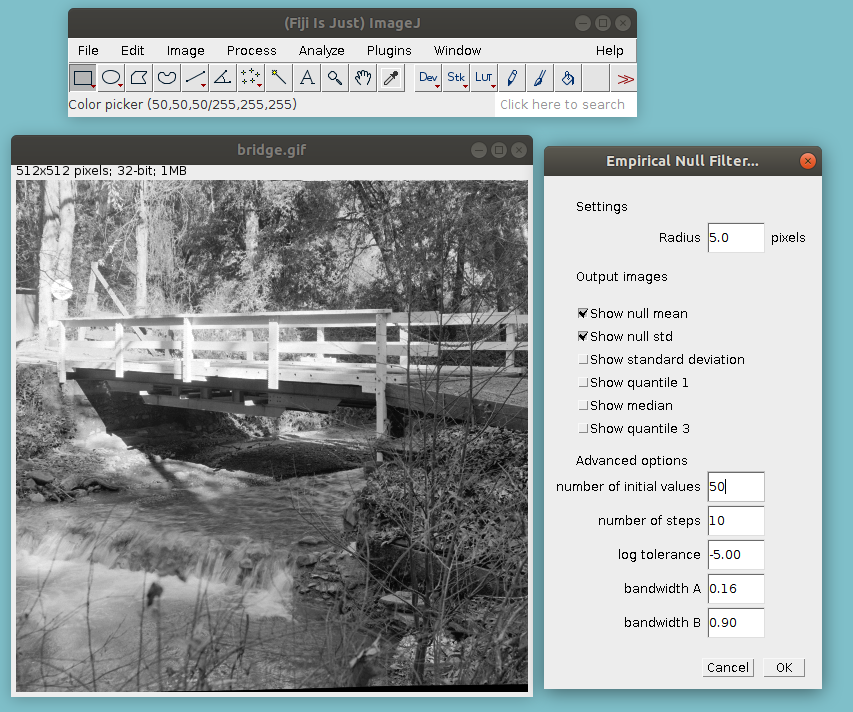
\includegraphics[width=\textwidth]{../figures/inference/fiji/gui.png}
    \caption{Graphical user interface of the empirical null filter in \texttt{Fiji}. The user can adjust the kernel radius as well as other advanced options relating to the Newton-Raphson method and the kernel density estimate. By products such as the empirical null parameters can be shown after the filtering as well.}
    \label{fig:inference_fijiGui}
\end{figure}

As a test, the empirical null filter with $r=5$ was used on a \texttt{ImageJ} sample image \texttt{bridge.gif}, as shown in Figure \ref{fig:inference_fijiBridgeFilter}. It is meaningless to use the empirical null filter on an image not for the purpose of the filter, however it does verify the filter works on arbitrary images. The empirical null images $\widehat{\mu}_{0,x,y}$ and $\widehat{\sigma}_{0,x,y}$ for all ${x,y}$ could be of interest. In particular the empirical null mean image could be interpreted as the result of a mode filter \citep{griffin2000mean}. Figure \ref{fig:inference_fijiMean} compares the empirical null mean with other averaging filters. The empirical null mean creates an impasto look and preserve edges which is similar to the result in \cite{griffin2000mean}. Spread filters such as the standard deviation filter can be used to detect edges. Figure \ref{fig:inference_fijiStd} compares the standard deviation filter with the empirical null standard deviation. The resulting images are similar but it was notable that the edges in the empirical null standard deviation are sharper, suggesting that the empirical null standard deviation is a more robust measure of spread compared to the standard deviation.

\begin{figure}
	\centering
    \centerline{
    \begin{subfigure}[b]{0.49\textwidth}
        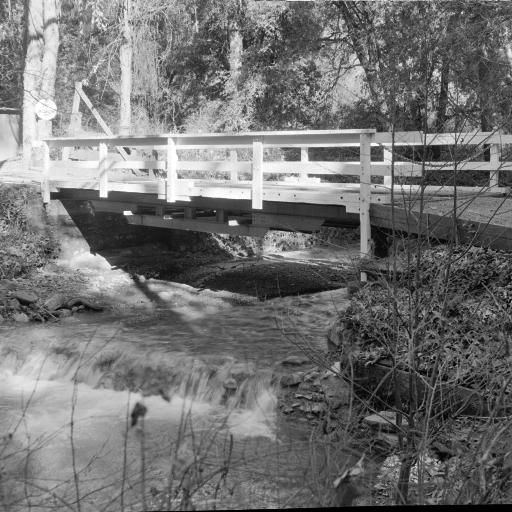
\includegraphics[width=\textwidth]{../figures/inference/fiji/bridge.png}
        \caption{Before filtering}
    \end{subfigure}
    \begin{subfigure}[b]{0.49\textwidth}
        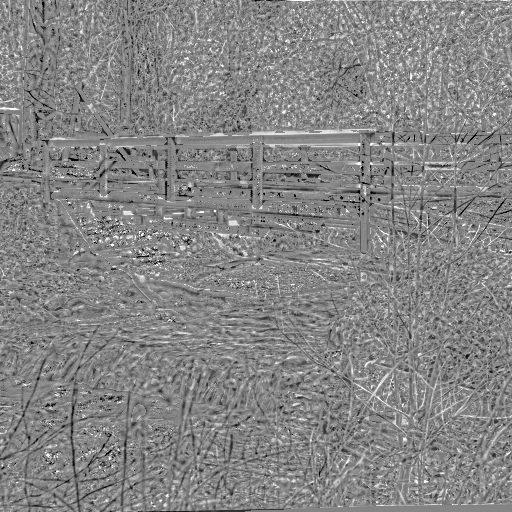
\includegraphics[width=\textwidth]{../figures/inference/fiji/bridgeFilter.png}
        \caption{After filtering}
    \end{subfigure}
    }
    \caption{Empirical null filter with $r=5$ on the sample image \texttt{bridge.gif}.}
    \label{fig:inference_fijiBridgeFilter}
\end{figure}

\begin{figure}
	\centering
    \centerline{
    \begin{subfigure}[b]{0.49\textwidth}
        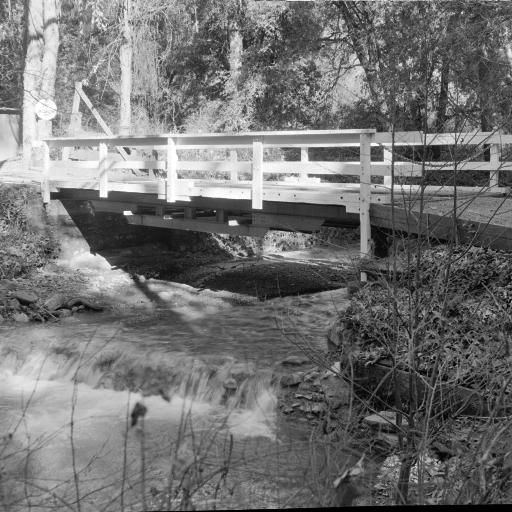
\includegraphics[width=\textwidth]{../figures/inference/fiji/bridge.png}
        \caption{No filter}
    \end{subfigure}
    \begin{subfigure}[b]{0.49\textwidth}
        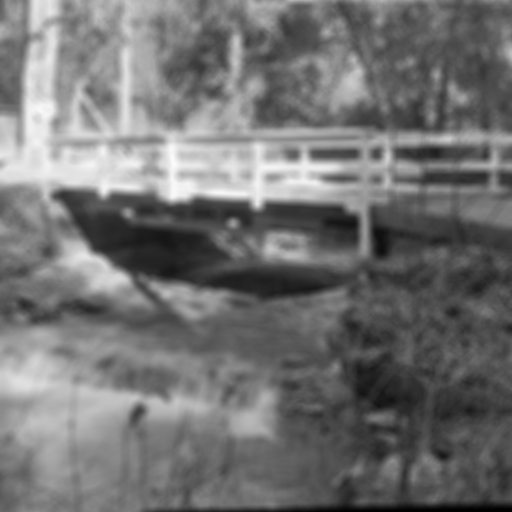
\includegraphics[width=\textwidth]{../figures/inference/fiji/mean.png}
        \caption{Mean filter}
    \end{subfigure}
    }
    \centerline{
    \begin{subfigure}[b]{0.49\textwidth}
        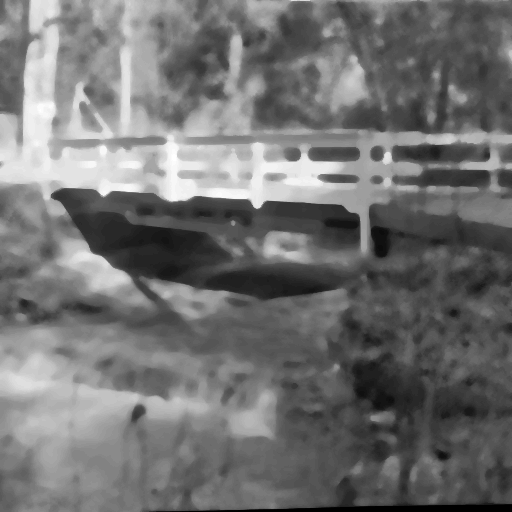
\includegraphics[width=\textwidth]{../figures/inference/fiji/median.png}
        \caption{Median filter}
    \end{subfigure}
    \begin{subfigure}[b]{0.49\textwidth}
        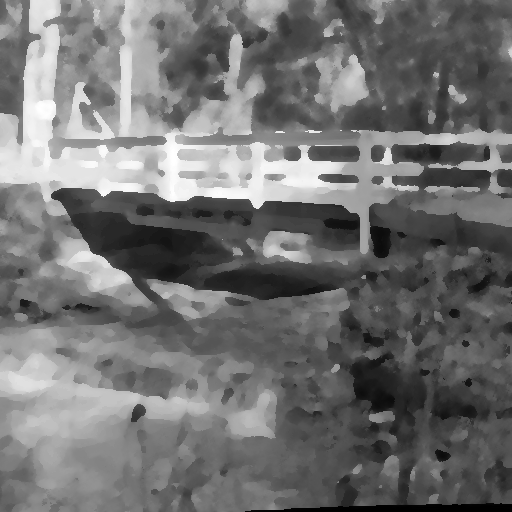
\includegraphics[width=\textwidth]{../figures/inference/fiji/nullMean.png}
        \caption{Empirical null mean}
    \end{subfigure}
    }
    \caption{Various average filters with kernel radius $r=5$ on the sample image \texttt{bridge.gif}}
    \label{fig:inference_fijiMean}
\end{figure}

\begin{figure}
	\centering
    \centerline{
    \begin{subfigure}[b]{0.49\textwidth}
        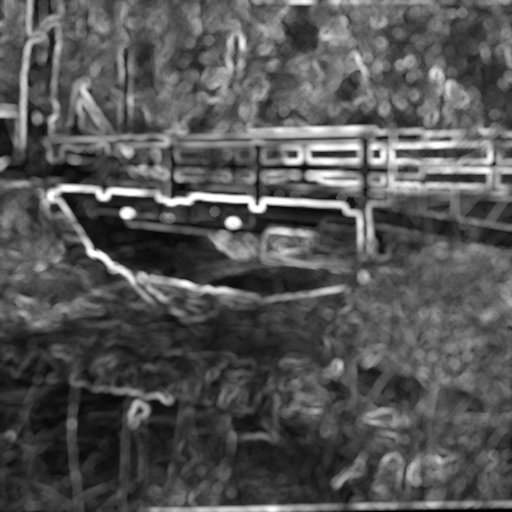
\includegraphics[width=\textwidth]{../figures/inference/fiji/std.png}
        \caption{Standard deviation filter}
    \end{subfigure}
    \begin{subfigure}[b]{0.49\textwidth}
        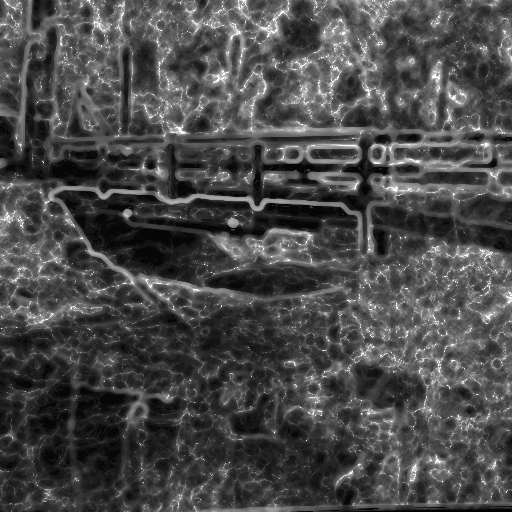
\includegraphics[width=\textwidth]{../figures/inference/fiji/nullStd.png}
        \caption{Empirical null standard deviation}
    \end{subfigure}
    }
    \caption{Various spread filters with kernel radius $r=5$ on the sample image \texttt{bridge.gif}.}
    \label{fig:inference_fijiStd}
\end{figure}

\subsection{Design and Implementation}

When using the the empirical null filter in \texttt{ImageJ}, the user is presented with a menu, as shown in Figure \ref{fig:inference_fijiGui}. Here the user can input the kernel radius, the filter then modifies the currently selected image $z_{x,y}$ to $\zeta_{x,y}$ for all $x$ and $y$ using a circular kernel with the specified radius. The menu also has options for by product images to be shown such as: the empirical null mean $\widehat{\mu}_{0,x,y}$, the empirical null standard deviation $\widehat{\sigma}_{0,x,y}$, the standard deviation filter, and quartile filters. Advanced options are available to the user. The number of initial values set the number of valid solutions to be found in the Newton-Raphson method on finding the mode of the density estimate, the solution with the gradient closest to zero is then used in further calculations. The user can also set the maximum number of steps and tolerance for the Newton-Raphson method. The bandwidth parameters for the kernel density estimate can also be adjusted here.

Because the empirical null filter was implemented by modifying the existing code in the class \texttt{RankFilters}, most of the design has already been done. \texttt{RankFilters} contain implementations of filters such as the mean filter and median filter. The implementation makes use of multiple threads, each thread filters a row in parallel. This is done by the following, a thread copies the value of each pixels in its current and neighbouring rows into a cache. Then for each column, the thread does calculations using the cache then replaces the pixel value of the image to be filtered. Once the row has been filtered, the thread then moves onto the next unfiltered row. Rows in the cache not needed are overwritten with more recent rows.

When the kernel captures pixels outside the boundary of the image or region of interest (ROI), \texttt{RankFilters} uses nearest pixel padding which fills in pixels outside the ROI with values to the nearest pixels. Figure \ref{fig:inference_padding_nearest} shows an example of nearest pixel padding on the top left corner of a rectangle ROI. This is not suitable for the empirical null filter as this will cause bias in a lot of calculations, especially the density fitting. The empirical null filter uses \texttt{NaN} padding which fills pixels outside the ROI with \texttt{NaN}. This indicate that these pixels are outside the ROI and are ignored. The number of non-\texttt{NaN} captured by the kernel is kept track for calculations such as the bandwidth for the kernel density estimate.

\begin{figure}
	\centering
	\begin{subfigure}[b]{0.49\textwidth}
	    \begin{tabular}{lllllll}
	       $\ddots$ & $\vdots$ & $\vdots$ & $\vdots$ & $\vdots$ & $\udots$ \\
	       $\cdots$ & $z_{1,1}$ & $z_{1,1}$ & $z_{1,1}$ & $z_{1,2}$ & $\cdots$ \\
	       $\cdots$ & $z_{1,1}$ & $z_{1,1}$ & $z_{1,1}$ & $z_{1,2}$ & $\cdots$ \\ \cline{4-6}
	       $\cdots$ & $z_{1,1}$ & \multicolumn{1}{l|}{$z_{1,1}$} & $z_{1,1}$ & $z_{1,2}$ & $\cdots$ \\
	       $\cdots$ & $z_{2,1}$ & \multicolumn{1}{l|}{$z_{2,1}$}  & $z_{2,1}$ & $z_{2,2}$ & $\cdots$ \\
	       $\udots$ & $\vdots$ & \multicolumn{1}{l|}{$\vdots$}  & $\vdots$ & $\vdots$ & $\ddots$
		\end{tabular}
		\caption{Nearest pixel padding}
		\label{fig:inference_padding_nearest}
	\end{subfigure}
	\begin{subfigure}[b]{0.49\textwidth}
	    \begin{tabular}{lllllll}
	       $\ddots$ & $\vdots$ & $\vdots$ & $\vdots$ & $\vdots$ & $\udots$ \\
	       $\cdots$ & \texttt{NaN} & \texttt{NaN} & \texttt{NaN} & \texttt{NaN} & $\cdots$ \\
	       $\cdots$ & \texttt{NaN} & \texttt{NaN} & \texttt{NaN} & \texttt{NaN} & $\cdots$ \\ \cline{4-6}
	       $\cdots$ & \texttt{NaN} & \multicolumn{1}{l|}{\texttt{NaN}} & $z_{1,1}$ & $z_{1,2}$ & $\cdots$ \\
	       $\cdots$ & \texttt{NaN} & \multicolumn{1}{l|}{\texttt{NaN}}  & $z_{2,1}$ & $z_{2,2}$ & $\cdots$ \\
	       $\udots$ & $\vdots$ & \multicolumn{1}{l|}{$\vdots$}  & $\vdots$ & $\vdots$ & $\ddots$
		\end{tabular}
		\caption{\texttt{NaN} padding}
		\label{fig:inference_padding_nan}
	\end{subfigure}
	\caption{When a kernel contain pixels outside the region of interest as shown by the solid line, the missing pixels can either be extrapolated using the nearest pixel or completely ignored by filling in the missing pixels with \texttt{NaN}.}
	\label{fig:inference_padding}
\end{figure}

Line filtering is done from left to right. At the start on the far left, an initial value of the median of all the pixels in the kernel is used. In addition, various initial values are randomly tried out until a requested number of valid solutions are found, the solution with the gradient closest to zero is used. For the following pixel to the right, the empirical null mean of the neighbouring left pixel is used as a initial point. This was chosen as it was assumed the empirical null mean would vary slowly and smoothly spatially.

Trying out more initial values is an advantage because it eliminates the chances of obtaining a sub-optimal solution such as a local maxima. However this is traded for computational cost. Additional initial values were generated by sampling from the Normal distribution centred on the first initial value and with standard deviation the same as the standard deviation using all pixels in the kernel.

\subsection{Uncontaminated Experiment}

The empirical null filter was demonstrated on an image where each pixel has i.i.d.~$\normal(0,1)$ test statistics. The test statistics after filtering should preserve its original distribution, or at least close to it. An experiment was conducted to investigate the empirical properties when filtering such as an image.

An example of a  $\addNumber{../figures/inference/noContamination/imageSize.txt}\times \addNumber{../figures/inference/noContamination/imageSize.txt}$ Gaussian image before and after filtering, with a kernel radius of \addNumber{../figures/inference/noContamination/radius.txt}, is shown in Figure \ref{fig:inference_noContamination_images}. A quick glance shows little difference, in particular the QQ plot in Figure \ref{fig:inference_noContamination_qq} shows that the post filter test statistics looked reasonably Normal. Because the empirical null mean and empirical null standard deviation are random variables with some distribution, the post filtered test statistics will never be Normal and any Normality tests would be too strict for the purpose of this experiment.

\begin{figure}[htp]
	\centering
	\includegraphics[width=0.49\textwidth]{../figures/inference/noContamination/allNullGaussianqq.eps}
	\caption{QQ plot of the test statistics of a filtered $\addNumber{../figures/inference/noContamination/imageSize.txt} \times \addNumber{../figures/inference/noContamination/imageSize.txt}$ Gaussian image after filtering with kernel radius \addNumber{../figures/inference/noContamination/radius.txt}.}
	\label{fig:inference_noContamination_qq}
\end{figure}

\begin{figure}[pht]
	\centering
	\centerline{
	\begin{subfigure}[b]{0.49\textwidth}
		\includegraphics[width=\textwidth]{../figures/inference/noContamination/allNullGaussianunfiltered.eps}
		\caption{Unfiltered}
	\end{subfigure}
	\begin{subfigure}[b]{0.49\textwidth}
		\includegraphics[width=\textwidth]{../figures/inference/noContamination/allNullGaussianfiltered.eps}
		\caption{Filtered}
	\end{subfigure}
	}
	\centerline{
	\begin{subfigure}[b]{0.49\textwidth}
		\includegraphics[width=\textwidth]{../figures/inference/noContamination/allNullGaussiannullmean.eps}
		\caption{Empirical null mean}
	\end{subfigure}
	\begin{subfigure}[b]{0.49\textwidth}
		\includegraphics[width=\textwidth]{../figures/inference/noContamination/allNullGaussiannullstd.eps}
		\caption{Empirical null std}
	\end{subfigure}
	}
	\caption{A $\addNumber{../figures/inference/noContamination/imageSize.txt} \times \addNumber{../figures/inference/noContamination/imageSize.txt}$ Gaussian image before and after filtering with kernel radius \addNumber{../figures/inference/noContamination/radius.txt}. Also shown are the empirical null mean and empirical null std.}
	\label{fig:inference_noContamination_images}
\end{figure}

In this experiment, a Gaussian image of size $\addNumber{../figures/inference/allnull/Experiment_AllNullGaussianwidth.txt} \times \addNumber{../figures/inference/allnull/Experiment_AllNullGaussianheight.txt}$ was simulated. The sample mean and sample variance of the post filtered test statistics were recorded. This was repeated \addNumber{../figures/inference/allnull/Experiment_AllNullGaussiannrepeat.txt} times by simulating another Gaussian image. Various kernel radiuses from $r = \addNumber{../figures/inference/allnull/Experiment_AllNullGaussianradius1.txt}$ to $r = \addNumber{../figures/inference/allnull/Experiment_AllNullGaussianradiusend.txt}$ were investigated.

\begin{figure}[htp]
	\centering
	\begin{subfigure}[b]{0.49\textwidth}
		\includegraphics[width=\textwidth]{../figures/inference/allnull/Experiment_AllNullGaussianmean.eps}
		\caption{Post filter sample mean}
	\end{subfigure}
	\begin{subfigure}[b]{0.49\textwidth}
		\includegraphics[width=\textwidth]{../figures/inference/allnull/Experiment_AllNullGaussianvariance.eps}
		\caption{Post filter sample variance}
	\end{subfigure}
	\caption{The sample mean and sample variance of the test statistics in a filtered Gaussian image of size $\addNumber{../figures/inference/allnull/Experiment_AllNullGaussianwidth.txt} \times \addNumber{../figures/inference/allnull/Experiment_AllNullGaussianheight.txt}$. The box plots summarise the \addNumber{../figures/inference/allnull/Experiment_AllNullGaussiannrepeat.txt} repeats of the experiment. The dotted lines show the critical region at the 2$\sigma$ level using standard tests for the sample mean and sample variance, assuming independence.}
	\label{fig:inference_allnullgaussian}
\end{figure}

The results are shown in Figure \ref{fig:inference_allnullgaussian}. The post filter sample test statistic means do agree with zero as expected. There is some bias with the post filter sample test statistics variances, it was found that this was sensitive to the bandwidth parameters for the kernel density estimate. The large sampling error can come from a number of sources. The empirical null parameters are random variables, thus correction using these can increase the variance. Also pixel to pixel correlation can be introduced as the empirical null parameters are functions of neighbouring pixels, this can contribute to the sample error.

It should be noted that the slight decrease of the post filter test statistic will decrease the sensitivity of the hypothesis test ever so slightly.

%\afterpage{\clearpage}
\subsection{Contaminated Experiment}

Consider a $\addNumber{../figures/inference/contamination/imageSize.txt}\times \addNumber{../figures/inference/contamination/imageSize.txt}$ Gaussian image with some contamination. For example let the pixels be $Z_{x,y}\sim\normal(\mu_{0,x,y},\sigma_0^2)$ where the null mean is a linear function
\begin{equation}
\mu_{0,x,y} = \addNumber{../figures/inference/contamination/gradx.txt} (x-x_0) + \addNumber{../figures/inference/contamination/grady.txt} (y-y_0)
\end{equation}
where $(x_0,y_0)$ is the centre of the image and $\sigma_0=\addNumber{../figures/inference/contamination/nullstd.txt}$. There are no defects or non-null pixels defined here, therefore any positive detections are false.

Figure \ref{fig:inference_contamination_images} shows an example of a contaminated image before and after filtering. When doing a hypothesis test, the contamination caused systematic error such that there are false positives on the two corners of the unfiltered image. The empirical null filter can recover the original image by extracting the systematic errors such as the plane, as shown by the empirical null mean, and the increase of variance, as shown by the empirical null std.

The QQ plot of the filtered test statistics, as shown in Figure \ref{fig:inference_contamination_qq}, shows that there may be a variance mismatch. A mismatch in the variance will increase or decrease the sensitivity of the test, a larger variance would increase the sensitivity.

\begin{figure}[htp]
	\centering
	\includegraphics[width=0.49\textwidth]{../figures/inference/contamination/allNullPlaneqq.eps}
	\caption{QQ plot of the test statistics of a filtered $\addNumber{../figures/inference/noContamination/imageSize.txt} \times \addNumber{../figures/inference/noContamination/imageSize.txt}$ contaminated Gaussian image after filtering with kernel radius \addNumber{../figures/inference/noContamination/radius.txt}.}
	\label{fig:inference_contamination_qq}
\end{figure}

\begin{figure}[pht]
	\centering
		\centerline{
			\begin{subfigure}[b]{0.49\textwidth}
				\includegraphics[width=\textwidth]{../figures/inference/contamination/allNullPlaneunfiltered.eps}
				\caption{Unfiltered}
			\end{subfigure}
			\begin{subfigure}[b]{0.49\textwidth}
				\includegraphics[width=\textwidth]{../figures/inference/contamination/allNullPlanefiltered.eps}
				\caption{Filtered}
			\end{subfigure}
		}
		\centerline{
			\begin{subfigure}{0.49\textwidth}
				\includegraphics[width=\textwidth]{../figures/inference/contamination/allNullPlanenullmean.eps}
				\caption{Empirical null mean}
			\end{subfigure}
			\begin{subfigure}{0.49\textwidth}
				\includegraphics[width=\textwidth]{../figures/inference/contamination/allNullPlanenullstd.eps}
				\caption{Empirical null std}
			\end{subfigure}
		}
	\caption{A $\addNumber{../figures/inference/contamination/imageSize.txt} \times \addNumber{../figures/inference/contamination/imageSize.txt}$ contaminated Gaussian image before and after filtering with kernel radius \addNumber{../figures/inference/contamination/radius.txt}. The contamination is such that the null distribution is $Z_{x,y}\sim\normal(\mu_{0,x,y},\sigma_0^2)$ where $\mu_{0,x,y} = \addNumber{../figures/inference/contamination/gradx.txt} (x-x_0) + \addNumber{../figures/inference/contamination/grady.txt} (y-y_0)$ and $\sigma_0=\addNumber{../figures/inference/contamination/nullstd.txt}$. Highlighted in red are significant pixels when controlling the FDR at the $2\sigma$ level. Also shown are the empirical null mean and empirical null std.}
	\label{fig:inference_contamination_images}
\end{figure}

An experiment was conducted to investigate the sample mean and sample variance of the filtered contaminated image. Ideally the sample mean and sample variance should be 0 and 1 respectively. Different radiuses were investigated from $r=\addNumber{../figures/inference/allnull/Experiment_AllNullPlaneradius1.txt}$ to $r=\addNumber{../figures/inference/allnull/Experiment_AllNullPlaneradiusend.txt}$ and repeated \addNumber{../figures/inference/allnull/Experiment_AllNullPlanenrepeat.txt} times.

The results are shown in Figure \ref{fig:inference_allnullplane}. The filter correctly centred the test statistics at zero. However there was some variance mismatch and this depended on the kernel radius. A kernel radius of about 80 scaled the test statistics correctly. This suggest there may be an optimal kernel radius for this particular null distribution. Another caveat is that the sensitivity may not be exactly preserved after filtering.

\begin{figure}[htp]
	\centering
	\begin{subfigure}[b]{0.49\textwidth}
		\includegraphics[width=\textwidth]{../figures/inference/allnull/Experiment_AllNullPlanemean.eps}
		\caption{Post filter sample mean}
	\end{subfigure}
	\begin{subfigure}[b]{0.49\textwidth}
		\includegraphics[width=\textwidth]{../figures/inference/allnull/Experiment_AllNullPlanevariance.eps}
		\caption{Post filter sample variance}
	\end{subfigure}
	\caption{The sample mean and sample variance of the test statistics in a filtered contaminated Gaussian image of size $\addNumber{../figures/inference/allnull/Experiment_AllNullGaussianwidth.txt} \times \addNumber{../figures/inference/allnull/Experiment_AllNullGaussianheight.txt}$. The contamination is such that the null distribution is $Z_{x,y}\sim\normal(\mu_{0,x,y},\sigma_0^2)$ where $\mu_{0,x,y} = \addNumber{../figures/inference/contamination/gradx.txt} (x-x_0) + \addNumber{../figures/inference/contamination/grady.txt} (y-y_0)$ and $\sigma_0=\addNumber{../figures/inference/contamination/nullstd.txt}$. The box plots summarise the \addNumber{../figures/inference/allnull/Experiment_AllNullPlanenrepeat.txt} repeats of the experiment. The dotted lines show the critical region at the 2$\sigma$ level using standard tests for the sample mean and sample variance, assuming independence.}
	\label{fig:inference_allnullplane}
\end{figure}

\subsection{Contaminated Defect Experiment}

The study will now turn to contaminated defected images. Let $Z_{x,y}$ be the test statistics of pixel $(x,y)$ and under the null, it is distributed such that $Z_{x,y}|H_0\sim\normal(0,1)$. Defects refer to statistics which do not follow the null distribution, but instead an alternative distribution. For example it can be $Z_{x,y}|H_1\sim\normal(\mu_{1,x,y},1)$ and this example was used in this experiment. Contamination is a linear transform of the test statistics $Z_{x,y}$ such that
\begin{equation}
	C_{x,y} = Z_{x,y}\sigma_{0,x,y} + \mu_{0,x,y} \ .
\end{equation}
The empirical null filter recovers $Z_{x,y}$ from $C_{x,y}$. The values of the filtered test statistics are denoted as $\zeta_{x,y}$.

Various simulated defects were investigated. Salt defect (named after salt and pepper noise) with density $\pi_1$ assign all test statistics to be distributed such that
\begin{equation}
	p_{Z_{x,y}}(z)=(1-\pi_1)p_{Z_{x,y}|H_0}(z) + \pi_1 p_{Z_{x,y}|H_1}(z) \ .
\end{equation}
In other words, test statistics will have the alternative distribution with probability $\pi_1$, and have the null distribution otherwise. This was chosen because the proportion of null statistics captured by a kernel should be independent of the radius of the kernel.

A line defect assign columns of pixels to have the alternative distribution, a kernel would only capture a section of defect. Similarly different shapes were used such as a square defect. With a square defect, a kernel can capture the entire defect.

An example of a salt defected image is shown in Figure \ref{fig:inference_saltDefect}, the figure also includes the image contaminated and filtered after contamination. The contamination caused some systematic errors, such as increasing the sensitivity such that are there more positive pixels in particular in two of the corners of the image. The empirical null filter recovers the defected image from the contaminated image so that appropriate inference can be done. However some statistical power is lost in the filtered image. This is because in areas of high empirical null std, the sensitivity decreased thus there is less detection power. This cannot be avoided as areas of high empirical null std is due to the sampling error. Using different kernel radiuses will change the sampling error of the empirical null std but it cannot be eliminated. Similar comments can be made for the line defect as shown in Figure \ref{fig:inference_lineDefect}.

The square defected images, including the contaminated ones, are shown in Figures \ref{fig:inference_squareDefect} and \ref{fig:inference_square2Defect}. Figure \ref{fig:inference_squareDefect} filtered the contaminated image using a kernel radius of $r=20$, while Figure \ref{fig:inference_square2Defect} used a kernel radius of $r=40$. With $r=20$, the kernel is smaller than the square defect, therefore the defect was treated as the null and this shows in the empirical null mean. This resulted in difficulty detecting the defect. With $r=40$, the kernel is much bigger than the defect and treated the defect as non-null. The empirical null filter recovers the gradient in the empirical null which was then used for inference.

\begin{figure}[p]
	\centering
		\centerline{
			\begin{subfigure}{0.49\textwidth}
				\includegraphics[width=\textwidth]{../figures/inference/defectsimulation/defectDust_imagePreContaminated.eps}
				\caption{Uncontaminated}
			\end{subfigure}
			\begin{subfigure}{0.49\textwidth}
				\includegraphics[width=\textwidth]{../figures/inference/defectsimulation/defectDust_imageContaminated.eps}
				\caption{Contaminated}
			\end{subfigure}
		}
		\centerline{
			\begin{subfigure}{0.49\textwidth}
				\includegraphics[width=\textwidth]{../figures/inference/defectsimulation/defectDust_imageFiltered.eps}
				\caption{Filtered}
			\end{subfigure}
			\begin{subfigure}{0.49\textwidth}
				\includegraphics[width=\textwidth]{../figures/inference/defectsimulation/defectDust_nullStd.eps}
				\caption{Empirical null std}
			\end{subfigure}
		}
	\caption{A $256 \times 256$ dust defect Gaussian image with/without contamination and after filtering with kernel radius 20. Defected pixels have the distribution $\normal(3,1)$. The salt defect has density $\pi_1 = 0.1$. The contamination is such that the null distribution is $Z_{x,y}\sim\normal(\mu_{0,x,y},\sigma_0^2)$ where $\mu_{0,x,y} = 0.01 (x-x_0) + 0.01 (y-y_0)$ and $\sigma_0=2$. Highlighted in red are significant pixels when controlling the FDR at the $2\sigma$ level.}
	\label{fig:inference_saltDefect}
\end{figure}

\begin{figure}[p]
	\centering
		\centerline{
			\begin{subfigure}{0.49\textwidth}
				\includegraphics[width=\textwidth]{../figures/inference/defectsimulation/defectLine_imagePreContaminated.eps}
				\caption{Uncontaminated}
			\end{subfigure}
			\begin{subfigure}{0.49\textwidth}
				\includegraphics[width=\textwidth]{../figures/inference/defectsimulation/defectLine_imageContaminated.eps}
				\caption{Contaminated}
			\end{subfigure}
		}
		\centerline{
			\begin{subfigure}{0.49\textwidth}
				\includegraphics[width=\textwidth]{../figures/inference/defectsimulation/defectLine_imageFiltered.eps}
				\caption{Filtered}
			\end{subfigure}
			\begin{subfigure}{0.49\textwidth}
				\includegraphics[width=\textwidth]{../figures/inference/defectsimulation/defectLine_nullStd.eps}
				\caption{Empirical null std}
			\end{subfigure}
		}
	\caption{A $256 \times 256$ line defect Gaussian image with/without contamination and after filtering with kernel radius 20. Defected pixels have the distribution $\normal(3,1)$. The line is 5 pixels thick. The contamination is such that the null distribution is $Z_{x,y}\sim\normal(\mu_{0,x,y},\sigma_0^2)$ where $\mu_{0,x,y} = 0.01 (x-x_0) + 0.01 (y-y_0)$ and $\sigma_0=2$. Highlighted in red are significant pixels when controlling the FDR at the $2\sigma$ level.}
	\label{fig:inference_lineDefect}
\end{figure}

\begin{figure}[p]
	\centering
		\centerline{
			\begin{subfigure}{0.49\textwidth}
				\includegraphics[width=\textwidth]{../figures/inference/defectsimulation/defectSquare_imagePreContaminated.eps}
				\caption{Uncontaminated}
			\end{subfigure}
			\begin{subfigure}{0.49\textwidth}
				\includegraphics[width=\textwidth]{../figures/inference/defectsimulation/defectSquare_imageContaminated.eps}
				\caption{Contaminated}
			\end{subfigure}
		}
		\centerline{
			\begin{subfigure}{0.49\textwidth}
				\includegraphics[width=\textwidth]{../figures/inference/defectsimulation/defectSquare_imageFiltered.eps}
				\caption{Filtered}
			\end{subfigure}
			\begin{subfigure}{0.49\textwidth}
				\includegraphics[width=\textwidth]{../figures/inference/defectsimulation/defectSquare_nullMean.eps}
				\caption{Empirical null mean}
			\end{subfigure}
		}
	\caption{A $256 \times 256$ square defect Gaussian image with/without contamination and after filtering with kernel radius 20. Defected pixels have the distribution $\normal(3,1)$. The square is $30\times 30$ pixels in size. The contamination is such that the null distribution is $Z_{x,y}\sim\normal(\mu_{0,x,y},\sigma_0^2)$ where $\mu_{0,x,y} = 0.01 (x-x_0) + 0.01 (y-y_0)$ and $\sigma_0=2$. Highlighted in red are significant pixels when controlling the FDR at the $2\sigma$ level.}
	\label{fig:inference_squareDefect}
\end{figure}

\begin{figure}[p]
	\centering
		\centerline{
			\begin{subfigure}{0.49\textwidth}
				\includegraphics[width=\textwidth]{../figures/inference/defectsimulation/defectSquare2_imagePreContaminated.eps}
				\caption{Uncontaminated}
			\end{subfigure}
			\begin{subfigure}{0.49\textwidth}
				\includegraphics[width=\textwidth]{../figures/inference/defectsimulation/defectSquare2_imageContaminated.eps}
				\caption{Contaminated}
			\end{subfigure}
		}
		\centerline{
			\begin{subfigure}{0.49\textwidth}
				\includegraphics[width=\textwidth]{../figures/inference/defectsimulation/defectSquare2_imageFiltered.eps}
				\caption{Filtered}
			\end{subfigure}
			\begin{subfigure}{0.49\textwidth}
				\includegraphics[width=\textwidth]{../figures/inference/defectsimulation/defectSquare2_nullMean.eps}
				\caption{Empirical null mean}
			\end{subfigure}
		}
	\caption{A $256 \times 256$ square defect Gaussian image with/without contamination and after filtering with kernel radius 40. Defected pixels have the distribution $\normal(3,1)$. The square is $30\times 30$ pixels in size. The contamination is such that the null distribution is $Z_{x,y}\sim\normal(\mu_{0,x,y},\sigma_0^2)$ where $\mu_{0,x,y} = 0.01 (x-x_0) + 0.01 (y-y_0)$ and $\sigma_0=2$. Highlighted in red are significant pixels when controlling the FDR at the $2\sigma$ level.}
	\label{fig:inference_square2Defect}
\end{figure}

The receiver operating characteristic (ROC) curves \citep{green1966signal, metz1978basic, hanley1982meaning, friedman2001elements, cook2007use} are shown in Figure \ref{fig:inference_defectSimulationRoc} for the various defects. The ROC curve is a parametric plot, plotting the true positive rate against the false positive rate for varying thresholds. Other authors \citep{metz1978basic} use terminology such as sensitivity and specificity. The area under the ROC curve is a commonly used statistic to quantify the performance of the test \citep{friedman2001elements}. Interpretations of the area do exist \citep{metz1978basic,hanley1982meaning} and discussed thoroughly in \cite{cook2007use}. The area under the ROC curve was recorded for different intensity values of the defect.

\begin{figure}[htp]
	\centering
		\centerline{
			\begin{subfigure}{0.49\textwidth}
				\includegraphics[width=\textwidth]{../figures/inference/defectsimulation/defectDust_roc.eps}
				\caption{Dust defect $\pi_1=0.1$, $r=20$}
			\end{subfigure}
			\begin{subfigure}{0.49\textwidth}
				\includegraphics[width=\textwidth]{../figures/inference/defectsimulation/defectLine_roc.eps}
				\caption{5 pixels thick line defect, $r=20$}
			\end{subfigure}
		}
		\centerline{
			\begin{subfigure}{0.49\textwidth}
				\includegraphics[width=\textwidth]{../figures/inference/defectsimulation/defectSquare_roc.eps}
				\caption{$30\times 30$ square defect, $r=20$}
				\label{fig:inference_defectSimulationRoc_square20}
			\end{subfigure}
			\begin{subfigure}{0.49\textwidth}
				\includegraphics[width=\textwidth]{../figures/inference/defectsimulation/defectSquare2_roc.eps}
				\caption{$30\times 30$ square defect, $r=40$}
			\end{subfigure}
		}
	\caption{ROC curves for various defected $256\times 256$ Gaussian images. The difference curves show the results for the non-contaminated image, contaminated image, and filtered contaminated image. Defected pixels have the distribution $\normal(3,1)$. The contamination is such that the null distribution is $Z_{x,y}\sim\normal(\mu_{0,x,y},\sigma_0^2)$ where $\mu_{0,x,y} = 0.01 (x-x_0) + 0.01 (y-y_0)$ and $\sigma_0=2$.}
	\label{fig:inference_defectSimulationRoc}
\end{figure}

In terms of the area under the ROC curves, the empirical null filter improves the performance over using the unfiltered contaminated image. The performance before contamination cannot be recovered but it is an improvement. For kernel radiuses too small, such as Figure \ref{fig:inference_defectSimulationRoc_square20}, the empirical null filter deteriorates the performance dramatically and it would be better off using the contaminated image.

The ROC is useful because it considers all thresholds or sensitivities used in the hypothesis testing. However in the previous experiment, it was found there was some variance mismatch before and after filtering with regards to the test statistics. As a result, for a given threshold, such as controlling the FDR, the sensitivity may change ever so slightly after filtering.

An experiment was conducted to investigate the sensitivity before and after filtering. A $256\times 256$ Gaussian image with dust defect of density $\pi_1=0.1$ was investigated. A kernel radius of $r=20$ was used. The type 1 error, type 2 error and the FDR were investigated before contamination, after contamination and after filtering for various alternative distribution. The alternative distribution used is $Z_{x,y}|H_1\sim\normal(\mu_1,1)$ where $\mu_1$ is the alternative mean and was varied for this experiment.

\begin{figure}[htp]
	\centering
		\centerline{
			\begin{subfigure}{0.49\textwidth}
				\includegraphics[width=\textwidth]{../figures/inference/defectsimulation/Experiment_DefectSimulationDust_roc.eps}
				\caption{ROC area}
			\end{subfigure}
			\begin{subfigure}{0.49\textwidth}
				\includegraphics[width=\textwidth]{../figures/inference/defectsimulation/Experiment_DefectSimulationDust_type1.eps}
				\caption{Type 1 error}
			\end{subfigure}
		}
		\centerline{
			\begin{subfigure}{0.49\textwidth}
				\includegraphics[width=\textwidth]{../figures/inference/defectsimulation/Experiment_DefectSimulationDust_type2.eps}
				\caption{Type 2 error}
			\end{subfigure}
			\begin{subfigure}{0.49\textwidth}
				\includegraphics[width=\textwidth]{../figures/inference/defectsimulation/Experiment_DefectSimulationDust_fdr.eps}
				\caption{FDR}
				\label{fig:inference_DefectSimulationDust_fdr}
			\end{subfigure}
		}
	\caption{ROC area and various errors obtained when conducting hypothesis test on the uncontaminated image, contaminated image and the filtered contaminated image of a $256 \times 256$ salt defect, Gaussian image. The filter used a kernel radius \addNumber{../figures/inference/defectsimulation/Experiment_DefectSimulationDust_radius.txt}. Defected pixels have the distribution $\normal(\mu_1,1)$ where $\mu_1$ was varied in this experiment. The salt defect has density $\pi_1 = 0.1$. The contamination is such that the null distribution is $Z_{x,y}\sim\normal(\mu_{0,x,y},\sigma_0^2)$ where $\mu_{0,x,y} = 0.01 (x-x_0) + 0.01 (y-y_0)$ and $\sigma_0=2$. The FDR was controlled at the $2\sigma$ level. The box plot summarise the \addNumber{../figures/inference/defectsimulation/Experiment_DefectSimulationDust_nRepeat.txt} repeats of the experiment. Some contamination plots may have been omitted due to being off the scale.}
	\label{fig:inference_DefectSimulationDust}
\end{figure}

The results are shown in Figure \ref{fig:inference_DefectSimulationDust}. The ROC areas were quantified here and shows that, in terms of the ROC area, using the filter improved the performance of the test from the contamination. Figure \ref{fig:inference_DefectSimulationDust_fdr} illustrate that in the uncontaminated image, the FDR is controlled below 5\%. However after contamination and then filtering, the FDR was not well controlled at this threshold. Ideally the error rates before contamination and after filtering should be similar so that sensitivity is preserved after filtering. This should highlight that while performance can be recovered from contamination in terms of the ROC area, the FDR threshold may not be preserved.

There is also the question of what kernel size to choose for a given defect. Literature, such as \cite{efron2004large} and \cite{schwartzman2008empirical}, suggest that, as a rule of thumb, the proportion of non-null statistics should not be larger than $\pi_1=0.1$ to satisfy some assumptions made for the empirical null. Given the size of the defect, one could work out the minimum kernel radius by setting a threshold for the maximum proportion of the area of kernel which is a defect to 10\%. In other words for a kernel with radius $r$
\begin{equation}
0.1 > \dfrac{\text{maximum area of defect captured by the kernel}}{\text{area of kernel}} \ .
\end{equation}
For a $d \times d$ square defect this is
\begin{equation}
r > d \sqrt{\dfrac{10}{\pi}} \ .
\end{equation}
In the example of $d=30$, this is about $r>54$. For the line defect with thickness $d$, it can be involved because the maximum area of the line defect captured by the kernel is
\begin{equation}
2r^2
\left[
	\dfrac{d}{2r}\sqrt{1-\left(\dfrac{d}{2r}\right)^2}
	+\text{arcsin}\left(\dfrac{d}{2r}\right)
\right] \ .
\end{equation}
For $d=5$, the radius is about $r>32$. These are rules of thumb because the kernel won't be perfectly circular when used on a grid of pixels. It should be pointed out that the implementation can accept non-integer radiuses if desired.

\begin{figure}[p]
	\centering
		\centerline{
			\begin{subfigure}{0.49\textwidth}
				\includegraphics[width=\textwidth]{../figures/inference/defectsimulation/Experiment_DefectRadiusLine_roc.eps}
				\caption{ROC area}
			\end{subfigure}
			\begin{subfigure}{0.49\textwidth}
				\includegraphics[width=\textwidth]{../figures/inference/defectsimulation/Experiment_DefectRadiusLine_type1.eps}
				\caption{Type 1 error}
			\end{subfigure}
		}
		\centerline{
			\begin{subfigure}{0.49\textwidth}
				\includegraphics[width=\textwidth]{../figures/inference/defectsimulation/Experiment_DefectRadiusLine_type2.eps}
				\caption{Type 2 error}
			\end{subfigure}
			\begin{subfigure}{0.49\textwidth}
				\includegraphics[width=\textwidth]{../figures/inference/defectsimulation/Experiment_DefectRadiusLine_fdr.eps}
				\caption{FDR}
			\end{subfigure}
		}
	\caption{ROC area and various errors obtained when conducting hypothesis test on the filtered contaminated image of a $256 \times 256$ line defected Gaussian image using various kernel radiuses. The dotted lines show the 95\% percentile when the hypothesis test was done on the uncontaminated image. Defected pixels have the distribution $\normal(\addNumber{../figures/inference/defectsimulation/Experiment_DefectRadiusLine_altMean.txt},1)$. The line defect is 5 pixels thick. The contamination is such that the null distribution is $Z_{x,y}\sim\normal(\mu_{0,x,y},\sigma_0^2)$ where $\mu_{0,x,y} = 0.01 (x-x_0) + 0.01 (y-y_0)$ and $\sigma_0=2$. The FDR was controlled at the $2\sigma$ level. The box plot summarise the \addNumber{../figures/inference/defectsimulation/Experiment_DefectRadiusLine_nRepeat.txt} repeats of the experiment.}
	\label{fig:inference_Experiment_DefectRadiusLine}
\end{figure}

\begin{figure}[p]
	\centering
		\centerline{
			\begin{subfigure}{0.49\textwidth}
				\includegraphics[width=\textwidth]{../figures/inference/defectsimulation/Experiment_DefectRadiusSquare_roc.eps}
				\caption{ROC area}
			\end{subfigure}
			\begin{subfigure}{0.49\textwidth}
				\includegraphics[width=\textwidth]{../figures/inference/defectsimulation/Experiment_DefectRadiusSquare_type1.eps}
				\caption{Type 1 error}
			\end{subfigure}
		}
		\centerline{
			\begin{subfigure}{0.49\textwidth}
				\includegraphics[width=\textwidth]{../figures/inference/defectsimulation/Experiment_DefectRadiusSquare_type2.eps}
				\caption{Type 2 error}
			\end{subfigure}
			\begin{subfigure}{0.49\textwidth}
				\includegraphics[width=\textwidth]{../figures/inference/defectsimulation/Experiment_DefectRadiusSquare_fdr.eps}
				\caption{FDR}
			\end{subfigure}
		}
	\caption{ROC area and various errors obtained when conducting hypothesis test on the filtered contaminated image of a $256 \times 256$ square defected Gaussian image using various kernel radiuses. The dotted lines show the 95\% percentile when the hypothesis test was done on the uncontaminated image. Defected pixels have the distribution $\normal(\addNumber{../figures/inference/defectsimulation/Experiment_DefectRadiusSquare_altMean.txt},1)$. The square defect is $30\times 30$ pixels in size. The contamination is such that the null distribution is $Z_{x,y}\sim\normal(\mu_{0,x,y},\sigma_0^2)$ where $\mu_{0,x,y} = 0.01 (x-x_0) + 0.01 (y-y_0)$ and $\sigma_0=2$. The FDR was controlled at the $2\sigma$ level. The box plot summarise the \addNumber{../figures/inference/defectsimulation/Experiment_DefectRadiusSquare_nRepeat.txt} repeats of the experiment.}
	\label{fig:inference_Experiment_DefectRadiusSquare}
\end{figure}

An experiment was conducted where the contaminated defected image were filtered for various kernel radiuses for a fixed alternative distribution $\normal(3,1)$. Hypothesis testing was done on the uncontaminated and filtered contaminated image. The area under the ROC curve and various errors were recorded. Results for the line and square defect are shown in Figures \ref{fig:inference_Experiment_DefectRadiusLine} and \ref{fig:inference_Experiment_DefectRadiusSquare} respectively.

The results show that the ROC area increased with kernel radius. This does highlight that a kernel with a good radius can performance almost as though there was no contamination. For large kernel radius, the FDR becomes similar to the FDR obtained from the uncontaminated image. Thus it appears a large kernel radius helped preserve FDR control after filtering in these examples. However a large kernel radius does come at a computational cost. Choosing a kernel radius is a matter of trading computational cost with precise FDR control.

\subsection{Real Data}

\begin{figure}[htp]
	\centering
		\centerline{
			\begin{subfigure}{0.49\textwidth}
				\includegraphics[width=\textwidth]{../figures/inference/defectdetect/ExperimentDefectDetectSep16120deg_radius1_z.eps}
				\caption{$r=\addNumber{../figures/inference/defectdetect/ExperimentDefectDetectSep16120deg_radius1.txt}$}
			\end{subfigure}
			\begin{subfigure}{0.49\textwidth}
				\includegraphics[width=\textwidth]{../figures/inference/defectdetect/ExperimentDefectDetectSep16120deg_radius2_z.eps}
				\caption{$r=\addNumber{../figures/inference/defectdetect/ExperimentDefectDetectSep16120deg_radius2.txt}$}
			\end{subfigure}
		}
		\centerline{
			\begin{subfigure}{0.49\textwidth}
				\includegraphics[width=\textwidth]{../figures/inference/defectdetect/ExperimentDefectDetectSep16120deg_radius3_z.eps}
				\caption{$r=\addNumber{../figures/inference/defectdetect/ExperimentDefectDetectSep16120deg_radius3.txt}$}
			\end{subfigure}
			\begin{subfigure}{0.49\textwidth}
				\includegraphics[width=\textwidth]{../figures/inference/defectdetect/ExperimentDefectDetectSep16120deg_radius4_z.eps}
				\caption{$r=\addNumber{../figures/inference/defectdetect/ExperimentDefectDetectSep16120deg_radius4.txt}$}
			\end{subfigure}
		}
	\caption{Filtered $z$ image from the \texttt{Sep16 120deg} dataset. Various kernel radiuses were used.}
	\label{fig:inference_sep16120deg_zfiltered}
\end{figure}

\begin{figure}[p]
	\centering
		\centerline{
			\begin{subfigure}[b]{0.49\textwidth}
				\includegraphics[width=\textwidth]{../figures/inference/defectdetect/ExperimentDefectDetectSep16120deg_radius1_sig.eps}
				\caption{Image with sig.~pixels}
			\end{subfigure}
			\begin{subfigure}[b]{0.49\textwidth}
				\includegraphics[width=\textwidth]{../figures/inference/defectdetect/ExperimentDefectDetectSep16120deg_radius1_logp.eps}
				\caption{$-\log p$}
			\end{subfigure}
		}
		\centerline{
			\begin{subfigure}{0.49\textwidth}
				\includegraphics[width=\textwidth]{../figures/inference/defectdetect/ExperimentDefectDetectSep16120deg_radius1_nullMean.eps}
				\caption{Empirical null mean}
			\end{subfigure}
			\begin{subfigure}{0.49\textwidth}
				\includegraphics[width=\textwidth]{../figures/inference/defectdetect/ExperimentDefectDetectSep16120deg_radius1_nullStd.eps}
				\caption{Empirical null std}
			\end{subfigure}
		}
	\caption{Resulting inference when using the empirical null filter with radius $r=\addNumber{../figures/inference/defectdetect/ExperimentDefectDetectSep16120deg_radius1.txt}$. a) Highlighted in red are significant pixels when controlling the FDR at the $2\sigma$ level. b) $p$-values on the log scale. c) and d) Empirical null mean and std.}
	\label{fig:inference_sep16120deg_inference_radius1}
\end{figure}

\begin{figure}[p]
	\centering
		\centerline{
			\begin{subfigure}[b]{0.49\textwidth}
				\includegraphics[width=\textwidth]{../figures/inference/defectdetect/ExperimentDefectDetectSep16120deg_radius2_sig.eps}
				\caption{Image with sig.~pixels}
			\end{subfigure}
			\begin{subfigure}[b]{0.49\textwidth}
				\includegraphics[width=\textwidth]{../figures/inference/defectdetect/ExperimentDefectDetectSep16120deg_radius2_logp.eps}
				\caption{$-\log p$}
			\end{subfigure}
		}
		\centerline{
			\begin{subfigure}{0.49\textwidth}
				\includegraphics[width=\textwidth]{../figures/inference/defectdetect/ExperimentDefectDetectSep16120deg_radius2_nullMean.eps}
				\caption{Empirical null mean}
			\end{subfigure}
			\begin{subfigure}{0.49\textwidth}
				\includegraphics[width=\textwidth]{../figures/inference/defectdetect/ExperimentDefectDetectSep16120deg_radius2_nullStd.eps}
				\caption{Empirical null std}
			\end{subfigure}
		}
	\caption{Resulting inference when using the empirical null filter with radius $r=\addNumber{../figures/inference/defectdetect/ExperimentDefectDetectSep16120deg_radius2.txt}$. a) Highlighted in red are significant pixels when controlling the FDR at the $2\sigma$ level. b) $p$-values on the log scale. c) and d) Empirical null mean and std.}
	\label{fig:inference_sep16120deg_inference_radius2}
\end{figure}

\begin{figure}[p]
	\centering
		\centerline{
			\begin{subfigure}[b]{0.49\textwidth}
				\includegraphics[width=\textwidth]{../figures/inference/defectdetect/ExperimentDefectDetectSep16120deg_radius3_sig.eps}
				\caption{Image with sig.~pixels}
			\end{subfigure}
			\begin{subfigure}[b]{0.49\textwidth}
				\includegraphics[width=\textwidth]{../figures/inference/defectdetect/ExperimentDefectDetectSep16120deg_radius3_logp.eps}
				\caption{$-\log p$}
			\end{subfigure}
		}
		\centerline{
			\begin{subfigure}{0.49\textwidth}
				\includegraphics[width=\textwidth]{../figures/inference/defectdetect/ExperimentDefectDetectSep16120deg_radius3_nullMean.eps}
				\caption{Empirical null mean}
			\end{subfigure}
			\begin{subfigure}{0.49\textwidth}
				\includegraphics[width=\textwidth]{../figures/inference/defectdetect/ExperimentDefectDetectSep16120deg_radius3_nullStd.eps}
				\caption{Empirical null std}
			\end{subfigure}
		}
	\caption{Resulting inference when using the empirical null filter with radius $r=\addNumber{../figures/inference/defectdetect/ExperimentDefectDetectSep16120deg_radius3.txt}$. a) Highlighted in red are significant pixels when controlling the FDR at the $2\sigma$ level. b) $p$-values on the log scale. c) and d) Empirical null mean and std.}
	\label{fig:inference_sep16120deg_inference_radius3}
\end{figure}

\begin{figure}[p]
	\centering
		\centerline{
			\begin{subfigure}[b]{0.49\textwidth}
				\includegraphics[width=\textwidth]{../figures/inference/defectdetect/ExperimentDefectDetectSep16120deg_radius4_sig.eps}
				\caption{Image with sig.~pixels}
			\end{subfigure}
			\begin{subfigure}[b]{0.49\textwidth}
				\includegraphics[width=\textwidth]{../figures/inference/defectdetect/ExperimentDefectDetectSep16120deg_radius4_logp.eps}
				\caption{$-\log p$}
			\end{subfigure}
		}
		\centerline{
			\begin{subfigure}{0.49\textwidth}
				\includegraphics[width=\textwidth]{../figures/inference/defectdetect/ExperimentDefectDetectSep16120deg_radius4_nullMean.eps}
				\caption{Empirical null mean}
			\end{subfigure}
			\begin{subfigure}{0.49\textwidth}
				\includegraphics[width=\textwidth]{../figures/inference/defectdetect/ExperimentDefectDetectSep16120deg_radius4_nullStd.eps}
				\caption{Empirical null std}
			\end{subfigure}
		}
	\caption{Resulting inference when using the empirical null filter with radius $r=\addNumber{../figures/inference/defectdetect/ExperimentDefectDetectSep16120deg_radius4.txt}$. a) Highlighted in red are significant pixels when controlling the FDR at the $2\sigma$ level. b) $p$-values on the log scale. c) and d) Empirical null mean and std.}
	\label{fig:inference_sep16120deg_inference_radius4}
\end{figure}

The empirical null filter was applied to the \texttt{Sep16 120deg} image as shown at the start of the chapter. Figure \ref{fig:inference_sep16120deg_zfiltered} shows the filtered $z$ images for various kernel radiuses. For $r=\addNumber{../figures/inference/defectdetect/ExperimentDefectDetectSep16120deg_radius1.txt}$, the resulting $z$ image is smooth and treated everything as the null. When a large enough radius was used, the defects are highlighted by the higher $z$ statistics and everything else remain unchanged. Figures \ref{fig:inference_sep16120deg_inference_radius1} to \ref{fig:inference_sep16120deg_inference_radius4} shows the resulting inference along with the empirical null parameters. The figures shows that for large enough kernel radius, the filter irons out the false positives observed at the start of this chapter. All of the defects were successfully highlighted by the hypothesis test.

False positives were detected on the bottom right of the 3D printed sample. This is the result of the null distribution being bimodal where each face has a different distribution. Figure \ref{fig:inference_cornerSelect} illustrates this. The geometry of the faces and the kernel is such it results in one of the faces to be treated as non-null and then tested positive, falsely so.

\begin{figure}[htp]
	\centering
		\centerline{
			\begin{subfigure}[b]{0.49\textwidth}
				\includegraphics[width=\textwidth]{../figures/inference/defectdetect/cornerSelect.png}
				\caption{$z$ image with kernel of radius $r=120$}
			\end{subfigure}
			\begin{subfigure}[b]{0.49\textwidth}
				\includegraphics[width=\textwidth]{../figures/inference/defectdetect/cornerSelectHisto.png}
				\caption{Histogram of $z$ in the kernel}
			\end{subfigure}
		}
	\caption{A kernel of radius $r=120$ is placed over the bottom right of a unfiltered $z$ image. The histogram of the $z$ statistics captured by the kernel shows a bimodal distribution.}
	\label{fig:inference_cornerSelect}
\end{figure}

The false positives were tackled by manually segmenting the image further as shown in Figure \ref{fig:inference_segmentFurther}. It was segmented using the edges of the projection of the 3D printed object. The empirical null filter was then used on each segment independently, ignoring pixels outside the segment the filter is working on. The resulting filtered segments were stitched together to form the resulting filtered image. By using this method, the resulting inference is shown in Figure \ref{fig:inference_subroisep16120deg_inference_radius4}. It can be seen that the empirical null mean does change face to face, resulting in a clear boundary set by the edges. Most of false positives around the corners and edges have been eliminated.

\begin{figure}[htp]
	\centering
	\includegraphics[width=0.49\textwidth]{../figures/inference/defectdetect/segment.JPG}
	\caption{The $z$ was segmented further into 7 segments.}
	\label{fig:inference_segmentFurther}
\end{figure}

\begin{figure}[p]
	\centering
		\centerline{
			\begin{subfigure}[b]{0.49\textwidth}
				\includegraphics[width=\textwidth]{../figures/inference/defectdetect/ExperimentSubRoiDefectDetectSep16120deg_radius4_sig.eps}
				\caption{Image with sig.~pixels}
			\end{subfigure}
			\begin{subfigure}[b]{0.49\textwidth}
				\includegraphics[width=\textwidth]{../figures/inference/defectdetect/ExperimentSubRoiDefectDetectSep16120deg_radius4_logp.eps}
				\caption{$-\log p$}
			\end{subfigure}
		}
		\centerline{
			\begin{subfigure}{0.49\textwidth}
				\includegraphics[width=\textwidth]{../figures/inference/defectdetect/ExperimentSubRoiDefectDetectSep16120deg_radius4_nullMean.eps}
				\caption{Empirical null mean}
			\end{subfigure}
			\begin{subfigure}{0.49\textwidth}
				\includegraphics[width=\textwidth]{../figures/inference/defectdetect/ExperimentSubRoiDefectDetectSep16120deg_radius4_nullStd.eps}
				\caption{Empirical null std}
			\end{subfigure}
		}
	\caption{Resulting inference when using the empirical null filter, on each segment independently, with radius $r=\addNumber{../figures/inference/defectdetect/ExperimentSubRoiDefectDetectSep16120deg_radius4.txt}$. a) Highlighted in red are significant pixels when controlling the FDR at the $2\sigma$ level. The $z$ statistics from all segments were combined in the BH procedure. b) $p$-values on the log scale. c) and d) Empirical null mean and std.}
	\label{fig:inference_subroisep16120deg_inference_radius4}
\end{figure}


\begin{figure}[p]
	\centering
		\centerline{
			\begin{subfigure}[b]{0.49\textwidth}
				\includegraphics[width=\textwidth]{../figures/inference/NullIid/NullIidEmpirical_nullMean.eps}
				\caption{Empirical null}
			\end{subfigure}
			\begin{subfigure}[b]{0.49\textwidth}
				\includegraphics[width=\textwidth]{../figures/inference/NullIid/NullIidMadMode_nullMean.eps}
				\caption{MAD mode null}
			\end{subfigure}
		}
		\centerline{
			\begin{subfigure}{0.49\textwidth}
				\includegraphics[width=\textwidth]{../figures/inference/NullIid/NullIidMeanVar_nullMean.eps}
				\caption{Mean variance null}
			\end{subfigure}
			\begin{subfigure}{0.49\textwidth}
				\includegraphics[width=\textwidth]{../figures/inference/NullIid/NullIidMedianIqr_nullMean.eps}
				\caption{Median IQR null}
			\end{subfigure}
		}
	\caption{Different types of central tendency estimators were used on $\pi r^2$ $\normal(0,1)$ random variables. Shown are the sampling distributions from 100 repeats. The dotted lines show the 95\% confidence interval for the sample mean.}
\end{figure}

\begin{figure}[p]
	\centering
		\centerline{
			\begin{subfigure}[b]{0.49\textwidth}
				\includegraphics[width=\textwidth]{../figures/inference/NullIid/NullIidEmpirical_nullStd.eps}
				\caption{Empirical null}
			\end{subfigure}
			\begin{subfigure}[b]{0.49\textwidth}
				\includegraphics[width=\textwidth]{../figures/inference/NullIid/NullIidMadMode_nullStd.eps}
				\caption{MAD mode null}
			\end{subfigure}
		}
		\centerline{
			\begin{subfigure}{0.49\textwidth}
				\includegraphics[width=\textwidth]{../figures/inference/NullIid/NullIidMeanVar_nullStd.eps}
				\caption{Mean variance null}
			\end{subfigure}
			\begin{subfigure}{0.49\textwidth}
				\includegraphics[width=\textwidth]{../figures/inference/NullIid/NullIidMedianIqr_nullStd.eps}
				\caption{Median IQR null}
			\end{subfigure}
		}
	\caption{Different types of statistical dispersion estimators were used on $\pi r^2$ $\normal(0,1)$ random variables. Shown are the sampling distributions from 100 repeats. The dotted lines show the 95\% confidence interval for the sample variance.}
\end{figure}

\begin{figure}[p]
	\centering
		\centerline{
			\begin{subfigure}[b]{0.49\textwidth}
				\includegraphics[width=\textwidth]{../figures/inference/NullIid/NullIidEmpirical_zMean.eps}
				\caption{Empirical null}
			\end{subfigure}
			\begin{subfigure}[b]{0.49\textwidth}
				\includegraphics[width=\textwidth]{../figures/inference/NullIid/NullIidMadMode_zMean.eps}
				\caption{MAD mode null}
			\end{subfigure}
		}
		\centerline{
			\begin{subfigure}{0.49\textwidth}
				\includegraphics[width=\textwidth]{../figures/inference/NullIid/NullIidMeanVar_zMean.eps}
				\caption{Mean variance null}
			\end{subfigure}
			\begin{subfigure}{0.49\textwidth}
				\includegraphics[width=\textwidth]{../figures/inference/NullIid/NullIidMedianIqr_zMean.eps}
				\caption{Median IQR null}
			\end{subfigure}
		}
	\caption{$\pi r^2$ $\normal(0,1)$ random variables were simulated and then normalised using the different types of estimators. Shown are the mean of the normalised random variables. The dotted lines show the 95\% confidence interval for the sample mean. The box plots represent 100 repeats of the simulation.}
\end{figure}

\begin{figure}[p]
	\centering
		\centerline{
			\begin{subfigure}[b]{0.49\textwidth}
				\includegraphics[width=\textwidth]{../figures/inference/NullIid/NullIidEmpirical_zStd.eps}
				\caption{Empirical null}
			\end{subfigure}
			\begin{subfigure}[b]{0.49\textwidth}
				\includegraphics[width=\textwidth]{../figures/inference/NullIid/NullIidMadMode_zStd.eps}
				\caption{MAD mode null}
			\end{subfigure}
		}
		\centerline{
			\begin{subfigure}{0.49\textwidth}
				\includegraphics[width=\textwidth]{../figures/inference/NullIid/NullIidMeanVar_zStd.eps}
				\caption{Mean variance null}
			\end{subfigure}
			\begin{subfigure}{0.49\textwidth}
				\includegraphics[width=\textwidth]{../figures/inference/NullIid/NullIidMedianIqr_zStd.eps}
				\caption{Median IQR null}
			\end{subfigure}
		}
	\caption{$\pi r^2$ $\normal(0,1)$ random variables were simulated and then normalised using the different types of estimators. Shown are the standard deviation of the normalised random variables. The dotted lines show the 95\% confidence interval for the sample variance. The box plots represent 100 repeats of the simulation.}
\end{figure}

\begin{figure}[p]
	\centering
		\centerline{
			\begin{subfigure}[b]{0.49\textwidth}
				\includegraphics[width=\textwidth]{../figures/inference/NullIid/NullIidEmpirical_zKurtosis.eps}
				\caption{Empirical null}
			\end{subfigure}
			\begin{subfigure}[b]{0.49\textwidth}
				\includegraphics[width=\textwidth]{../figures/inference/NullIid/NullIidMadMode_zKurtosis.eps}
				\caption{MAD mode null}
			\end{subfigure}
		}
		\centerline{
			\begin{subfigure}{0.49\textwidth}
				\includegraphics[width=\textwidth]{../figures/inference/NullIid/NullIidMeanVar_zKurtosis.eps}
				\caption{Mean variance null}
			\end{subfigure}
			\begin{subfigure}{0.49\textwidth}
				\includegraphics[width=\textwidth]{../figures/inference/NullIid/NullIidMedianIqr_zKurtosis.eps}
				\caption{Median IQR null}
			\end{subfigure}
		}
	\caption{$\pi r^2$ $\normal(0,1)$ random variables were simulated and then normalised using the different types of estimators. Shown are the sample kurtosis of the normalised random variables. The dotted lines show the 95\% confidence interval for the sample kurtosis. The box plots represent 100 repeats of the simulation.}
\end{figure}

\begin{figure}[p]
	\centering
		\centerline{
			\begin{subfigure}[b]{0.49\textwidth}
				\includegraphics[width=\textwidth]{../figures/inference/NullIid/NullIidMixtureEmpirical_nullMean.eps}
				\caption{Empirical null}
			\end{subfigure}
			\begin{subfigure}[b]{0.49\textwidth}
				\includegraphics[width=\textwidth]{../figures/inference/NullIid/NullIidMixtureMadMode_nullMean.eps}
				\caption{MAD mode null}
			\end{subfigure}
		}
		\centerline{
			\begin{subfigure}{0.49\textwidth}
				\includegraphics[width=\textwidth]{../figures/inference/NullIid/NullIidMixtureMeanVar_nullMean.eps}
				\caption{Mean variance null}
			\end{subfigure}
			\begin{subfigure}{0.49\textwidth}
				\includegraphics[width=\textwidth]{../figures/inference/NullIid/NullIidMixtureMedianIqr_nullMean.eps}
				\caption{Median IQR null}
			\end{subfigure}
		}
	\caption{Different types of central tendency estimators were used on $\pi r^2$ mixture of Gaussian random variables. The random variable has distribution $\normal(0,1)$ with probability $0.9$ and $\normal(3,1)$ with probability $0.1$. Shown are the sampling distributions from 100 repeats. The dotted lines show the 95\% confidence interval for the sample mean.}
\end{figure}

\begin{figure}[p]
	\centering
		\centerline{
			\begin{subfigure}[b]{0.49\textwidth}
				\includegraphics[width=\textwidth]{../figures/inference/NullIid/NullIidMixtureEmpirical_nullStd.eps}
				\caption{Empirical null}
			\end{subfigure}
			\begin{subfigure}[b]{0.49\textwidth}
				\includegraphics[width=\textwidth]{../figures/inference/NullIid/NullIidMixtureMadMode_nullStd.eps}
				\caption{MAD mode null}
			\end{subfigure}
		}
		\centerline{
			\begin{subfigure}{0.49\textwidth}
				\includegraphics[width=\textwidth]{../figures/inference/NullIid/NullIidMixtureMeanVar_nullStd.eps}
				\caption{Mean variance null}
			\end{subfigure}
			\begin{subfigure}{0.49\textwidth}
				\includegraphics[width=\textwidth]{../figures/inference/NullIid/NullIidMixtureMedianIqr_nullStd.eps}
				\caption{Median IQR null}
			\end{subfigure}
		}
	\caption{Different types of statistical dispersion estimators were used on $\pi r^2$ mixture of Gaussian random variables. The random variable has distribution $\normal(0,1)$ with probability $0.9$ and $\normal(3,1)$ with probability $0.1$. Shown are the sampling distributions from 100 repeats. The dotted lines show the 95\% confidence interval for the sample variance.}
\end{figure}